% !TeX encoding = UTF-8
% !TeX program = pdfLaTeX
% !TeX root = matlab-exercises-emaip.tex
% !TeX spellcheck = en_GB
\documentclass[fleqn, 12pt,a4paper]{article}
\usepackage[colorlinks, linkcolor=blue, citecolor=blue, urlcolor=blue]{hyperref}
%\usepackage[nosolutionfiles]{answers}
\usepackage{answers}
\usepackage{graphicx}
\usepackage{amsmath}
\usepackage{todonotes}
\usepackage{fancyvrb}
\usepackage{xparse}
\usepackage{listings}
\usepackage{multicol}
\usepackage{tcolorbox}
\usepackage{wrapfig}
\usepackage{color}
\definecolor{dkgreen}{rgb}{0,0.6,0}
\definecolor{gray}{rgb}{0.5,0.5,0.5}

\lstset{language=Matlab,
   keywords={break,case,catch,continue,else,elseif,end,for,function,
      global,if,otherwise,persistent,return,switch,try,while},
   basicstyle=\footnotesize\ttfamily,
   keywordstyle=\color{blue},
   commentstyle=\color{dkgreen},
   stringstyle=\color{dkgreen},
%   numbers=left,
%   numberstyle=\tiny\color{gray},
%   stepnumber=3,
%   numbersep=10pt,
   backgroundcolor=\color{white},
   tabsize=4,
   showspaces=false,
   showstringspaces=false}

\newcommand{\moved}{\todo[inline]{The exercise above has been moved to matlab with unittests.}}


% Fix for moving the hypertarget one line up.
% https://tex.stackexchange.com/a/412381/1366
\makeatletter
 \newcommand{\linkdest}[1]{\Hy@raisedlink{\hypertarget{#1}{}}}
\makeatother

\newcounter{ex}
\numberwithin{ex}{section}

\newenvironment{ex}[1][]{%
%\filbreak
\medbreak
\refstepcounter{ex}
\noindent
\textbf{\linkdest{\theex{}exercise}{}Exercise \theex{}: #1\hfill\hyperlink{\theex{}hint}{hint}, \hyperlink{\theex{}solution}{solution}}\par\noindent}{}

\Newassociation{sol}{Solution}{ans}
\Newassociation{hint}{Hint}{hnt}


% Redefine the Hint and Solution environment.
\renewenvironment{Hint}[1]{{\filbreak\par\noindent\linkdest{#1{}hint}{}\bf Exercise \hyperlink{#1{}exercise}{#1}:}\newline}{\bigskip}
\renewenvironment{Solution}[1]{{\filbreak\par\noindent\linkdest{#1{}solution}{}\bf Exercise \hyperlink{#1{}exercise}{#1}:}\newline}{\bigskip}

\Opensolutionfile{ans}[ans]
\Opensolutionfile{hnt}[hints]

% Macros for writing solutions and unittests to files
% in the exercises subdirectory.

% The subdirectory to save exercises in.
\NewDocumentCommand{\CurrentExerciseDirectory}{}{00default}

% Command to update which directory to save files in.
\NewDocumentCommand{\SetExerciseDirectory}{m}{%
	\RenewDocumentCommand{\CurrentExerciseDirectory}{}{#1}}

% Automatically numbered files, with the filename
% structure exercise_2.2_plot.m
\NewDocumentEnvironment{solutionfile}{m}
  {\VerbatimOut{exercises/\CurrentExerciseDirectory/#1}}
  {\endVerbatimOut}
\NewDocumentEnvironment{testfile}{m}
  {\VerbatimOut{exercises/\CurrentExerciseDirectory/exercise_\theex_#1}}
  {\endVerbatimOut}


\author{Henrik Skov Midtiby}
\title{Matlab exercises for E-MAIP 2019}
\date{\today}

%\includeonly{}

\begin{document}
\maketitle

\newpage
\tableofcontents

\newpage
\section*{Introduction}

These notes are used in the course \emph{Mathematics and Introduction to programming}
that is taught on University of Southern Denmark during fall 2019.

The source for this document is available on github, 
\url{https://github.com/henrikmidtiby/matlab-notes}.


% !TeX encoding = UTF-8
% !TeX program = pdfLaTeX
% !TeX root = matlab-exercises-emaip.tex
% !TeX spellcheck = en_GB
\section{Setting git up on Windows}

In this section it is explained how to set up git on 
a Windows computer.
This is also described in this \href{https://tekvideo.sdu.dk/t/henrikmidtiby/E-MAIP-2020/2020/1/blok04/4}{video}.

The steps are as follows:
\begin{enumerate}
\item		Download and install \emph{Git for Windows} from \url{https://git-scm.com/}
\item		Open \emph{Git Bash} and identify yourself to git
\item		Generate an ssh key
\item 	Add the generated ssh key to \url{https://gitlab.sdu.dk}
\end{enumerate}

\subsection{Download and installation of \emph{Git for Windows}}

Open \url{https://git-scm.com/} and click on the download button
in the right side of the page.

\subsection{Open Git Bash and identify yourself to git}

Find the \emph{Git Bash} program and start it.
It will look like a black image with some coloured text in the 
top left corner.
What is opened now is a computer console or terminal.
It can be very effective to do certain tasks on the computer through the console.

To set name and email that the git installation uses on the 
computer, the following commands should be executed:
\begin{verbatim}
git config --global user.name "<your name>"
git config --global user.email "<your email>"
\end{verbatim}

For me it looked like this:
\begin{verbatim}
hemi@TEK-CB-HEMI-01 MINGW64 ~
$ git config --global user.name "Henrik Skov Midtiby"

hemi@TEK-CB-HEMI-01 MINGW64 ~
$ git config --global user.email "hemi@mmmi.sdu.dk"
\end{verbatim}

\subsection{Generate an ssh key}

To work efficiently with git on remote servers like \url{https://gitlab.sdu.dk} or \url{https://github.com}, you need to generate 
an ssh key.
In Git Bash it is done with the command.
\begin{verbatim}
ssh-keygen -t rsa
\end{verbatim}
After executing the command, the \emph{ssh-keygen} program
will ask you a few questions and then the ssh key is generated.
It is appropriate to use the default values, so you can just 
press enter to accept the default values.

On my computer the key generation process looked like this:
\begin{verbatim}
hemi@TEK-CB-HEMI-01 MINGW64 ~
$ ssh-keygen -t rsa
Generating public/private rsa key pair.
Enter file in which to save the key (/c/Users/hemi/.ssh/id_rsa):
Enter passphrase (empty for no passphrase):
Enter same passphrase again:
Your identification has been saved in /c/Users/hemi/.ssh/id_rsa
Your public key has been saved in /c/Users/hemi/.ssh/id_rsa.pub
The key fingerprint is:
SHA256:GBdcG4YGzNMGF9bOZ5oK7P+m+IxO1+8hYpT2g3g/+Ok hemi@TEK-CB-HEMI-01
The key's randomart image is:
+---[RSA 3072]----+
|     oo===+      |
|      +o*o.o     |
|      .+.o.      |
|       + .o o    |
|     .. S  =     |
|      o+ +o      |
|     .o.*o= .    |
|     ..Booo= .   |
|     .+o=*Eoo    |
+----[SHA256]-----+
\end{verbatim}

\subsection{Add ssh key to gitlab.sdu.dk}

As you have now generated an ssh key, you need to locate the 
public part of the key and add that to \url{https://gitlab.sdu.dk}.
This can be done with the following command.
\begin{verbatim}
cat <path to public key>
\end{verbatim}

On my computer the key is placed in this location 
\verb!/c/Users/hemi/.ssh/id_rsa.pub!, which was displayed 
in the output from the key generation step.

\begin{verbatim}
hemi@TEK-CB-HEMI-01 MINGW64 ~
$ cat /c/Users/hemi/.ssh/id_rsa.pub
ssh-rsa AAAAB3NzaC1yc2EAAAADAQABAAABgQCz0X6DyHeyiqcPe8Y+zeQ60Y
4F0sxR2MqNlsL52ZrllRd0toAFvPvmrz9/rT13eHoD+xSIQ5kL44GTZqn9fRmC
lG3ttc1v7Qd/KmAmM5eOpr+cH/c/IbfFGQyiRV7lRz5KES8TFUEs8YNLfLwdHU
cEhmn7x4Zmc7aahTQFTH55EqOt6HU5YoF4vMe0LG+WnhNrh/kwiKN1ndqasEC6
wE3D6K2/Z21j8FcFqvR0PWDubUABQdMN5+huQ7/O7SAVQCeZBYoG2fcn9HRu39
IS8kKQ3AmmrDFUitaWhIWZ+msfmTqJCplYXVlGrlvjcbIVPIgCr/4IL6soWE1V
KL1cEVGV2lAktMqP9cU1E6rYMFMtYIIyjSkE5l2YJZ++A+dgayHOqBx5qPXRq2
k2gRAz8auiV0ztOCRtA09IhzvlH0ZHU126ZoxC72BJpMP6+Rp3r8EJ4LlU2IaI
SXnoSAqXtc8HvngXm74TQpneLSDy+nMKZJ1jpL9dqxtWUM3DbhPyzaM= hemi@
TEK-CB-HEMI-01
\end{verbatim}


\subsection{Cloning a git repository}

Open a command line / terminal in the location where you
want to put a local copy of the git repository.
This can be done by right clicking on the folder in 
Pathfinder, Finder or Nautilus and selecting 
\emph{Git BASH here}, \emph{Open terminal} or something similar.
When the terminal is opened in the proper location, issue the 
command below to clone the specified git repository.
\begin{verbatim}
git clone git@gitlab.sdu.dk:midtiby/2020-emaip/
emaip-2020-exercises/emaip-exercises-studentid.git

\end{verbatim}


\subsection{Daily use of git}

The recommended working routine with git is 
described below.
At start of the day, the goal is to get current
with changes from other members of the team.
This is achieved by the commands.
\begin{verbatim}
git fetch
git rebase origin/master
git push
\end{verbatim}
If git complains about not knowing which repository to push
changes to, the following command will
set it up.

\begin{verbatim}
git push --set-upstream origin master
\end{verbatim}

 
% !TeX encoding = UTF-8
% !TeX program = pdfLaTeX
% !TeX root = matlab-exercises-emaip.tex
% !TeX spellcheck = en_GB
\section{Matlab introduction}
\todo[inline]{Add Matlab introduction exercises}
\todo[inline]{Add exercises about systems of linear equations}


\subsection{If statements}

\todo[inline]{Use this as inspiration for introducing if statements \url{https://www.learnbyexample.org/python-if-else-elif-statement/}¨}

\todo[inline]{Experiment with decision tables for specifying branching behaviour \url{https://www.hillelwayne.com/decision-tables/}}

\subsection{For loops}

Consider the task of adding all integers from 1 to 9
and storing the result in the variable \verb!val!;  
this can be achieved with the following code 
\begin{lstlisting}
val = 1 + 2 + 3 + 4 + 5 + 6 + 7 + 8 + 9
\end{lstlisting}
This is straightforward to write, but does not scale
as well as possible.
Adding all integers from 1 to 100 with a similar method
is still possible although impractical.
The task of adding all integers from 1 to 1000000 
is impractical, so lets look at better ways of doing such 
calculations.

The first step to make the code easier to write, does the
direct opposite thing; it makes the code much longer, but it 
also gives it a more repeating structure, which soon will be 
exploited 
\begin{lstlisting}
val = 0;
val = val + 1;
val = val + 2;
val = val + 3;
val = val + 4;
val = val + 5;
val = val + 6;
val = val + 7;
val = val + 8;
val = val + 9;
val
\end{lstlisting}
It still bothers me that the line where \verb!val! is updated
changes from line to line.
To avoid this a helper variable $k$ is introduced.
Before each update of \verb!val! the value of $k$ is 
increased by one and then the update rule can be used.
\begin{lstlisting}
val = 0;
k = 1;
val = val + k;
k = 2;
val = val + k;
k = 3;
val = val + k;
k = 4;
val = val + k;
k = 5;
val = val + k;
k = 6;
val = val + k;
k = 7;
val = val + k;
k = 8;
val = val + k;
k = 9;
val = val + k;
val
\end{lstlisting}
To tell matlab to repeat the update rule \verb!val = val + k! for
all values of $k$ from 1 to 9, the following code can be used:
\begin{lstlisting}
val = 0;
for k = 1:9
    val = val + k;
end
val
\end{lstlisting}
Compared with the first approach of manually typing
all the integers in the range 1 to 9, it takes a bit more space, 
but the code has become much easier to adapt to other problems.


\begin{ex}\label{exSumIntegersUp100}%
Determine the value of 
\begin{align*}
\sum_{k = 1}^{100} k = 1 + 2 + 3 + \ldots + 98 + 99 + 100
\end{align*}
In other words calculate the sum of all integers from 1 to 100.
\begin{hint}
A for loop will be a good structure to use.
The answer is 5050.
\end{hint}
\begin{sol}
A solution is:
\begin{lstlisting}
val = 0;
for k = 1:100
    val = val + k;
end
val
\end{lstlisting}
\end{sol}
\end{ex}

\begin{ex}
Determine the value of 
\begin{align*}
\sum_{k = 1}^{100} \sin(k) = \sin(1) + \sin(2) + \ldots + \sin(99) + \sin(100)
\end{align*}
\begin{hint}
A for loop will be a good structure to use.
The answer is -0.1272.
\end{hint}
\begin{sol}
A solution is:
\begin{lstlisting}
val = 0;
for k = 1:100
    val = val + sin(k);
end
val
\end{lstlisting}
\end{sol}
\end{ex}


\begin{ex}
Test the following expression by selecting a positive integer $n$
and evaluate both sides of the expression using the selected value.
\begin{align*}
\sum_{i = 1}^n i = \frac{n \cdot (n + 1)}{2}
\end{align*}
Repeat this with three different value of $n$.
\begin{hint}
Look at the code from exercise \ref{exSumIntegersUp100}.
It can be adapted to evaluate the left hand side of the expression.
\end{hint}
\begin{sol}
A solution is:
\begin{lstlisting}
n = 234;
val_left = 0;
for k = 1:n
    val_left = val_left + k;
end
val_left
val_right = n * (n + 1) / 2
\end{lstlisting}
\end{sol}
\end{ex}


\begin{ex}
Test the following expression by selecting a positive value $a$
which is not one and an integer $n$
and evaluate both sides of the expression using the selected value.
\begin{align*}
\sum_{i = 0}^n a^i = \frac{1 - a^{n + 1}}{1 - a}
\end{align*}
Repeat this with three different value of $n$.
\begin{hint}
Look at the code from exercise \ref{exSumIntegersUp100}.
It can be adapted to evaluate the left hand side of the expression.
\end{hint}
\begin{sol}
A solution is:
\begin{lstlisting}
a = 1.2;
n = 43;
val_left = 0;
for k = 0:n
    val_left = val_left + a^k;
end
val_left
val_right = (1 - a^(n + 1)) / (1 - a)
\end{lstlisting}
\end{sol}
\end{ex}


\subsection{While loops}

\todo[inline]{Write about code indentation \url{https://dev.to/sanjaysinghrajpoot/why-indentation-is-more-important-than-coding-4fn1}}

\subsection{Plot of secant lines}

\begin{ex}
Draw multiple secant lines on the same figure.
The distance between the points that define the secant line
should be reduced before plotting the next secant line.
Use the following distances between the $x$ values:
$h \in {0.2, 0.1, 0.05, 0.02, 0.01}$.
Please use the template below
\begin{lstlisting}
% Create x values
x = linspace(-3, 6, 100);

% Create a function handle for the function to plot.
fh = @(x) 2*x.^2 - x + 1;

% Find the two end points of the secant to plot.
h = 2;
x0 = 0.2;
x1 = x0 + h;
y0 = fh(x0);
y1 = fh(x1);

% Open a figure and plot the x and y values.
figure(2);
hold off;
% Plot the function
plot(x, fh(x));
hold on;
plot([x0, x1], [y0, y1], 'o-');
\end{lstlisting}
\begin{hint}
\end{hint}
\begin{sol}
A solution is:
\begin{lstlisting}
\end{lstlisting}
\end{sol}
\end{ex}

%
%%% Indskrive vektorer og matricer
%A = [1, 2, 3; 2, 3, 1; 1, 1, 1]
%B = [1, 1, 1; 1, 2, 4; 7, 6, 5]
%C = [1; 2; 3]
%
%
%%% Addition
%disp('addition');
%A + A
%A + B
%B + A
%B + B
%
%
%%% Multiplikation
%disp('multiplikation');
%A * A
%A * B
%B * A
%B * B
%
%
%%% 
%% Transponering
%A
%transpose(A)
%A'
%
%
%%% Opgave
%% Find nogle opgaver med matricer og vektorer.
%% Tjek jeres resultater ved at få Matlab til at udføre de samme beregninger
%% som I har gjort i hånden.
%
%
%
%%%
%% Løsning af lineære ligningssystemer
%
%% Givet ligningerne
%% 2*x1 + 5*x2 = 2 og -4*x1+3*x2 = -30.
%% Kan koefficient matricen A og værdi vektoren b opskrives.
%A = [2, 5; -4, 3];
%b = [2; -30];
%
%% Ud fra værdi vektoren og koefficient matricen, kan 
%% løsningen til ligningssystemet bestemmes på følgende 
%% tre forskellige måder.
%A \ b
%inv(A) * b
%linsolve(A, b)
%
%
%%%
%% Opgave
%% Plot ligningerne x + 2y = 3 og 2x - y = 2 i det samme 
%% koordinatsystem.
%% Opskriv ligningsystemet på matrix form og løs det via 
%% linsolve eller lign.
%% Plot løsningen sammen med de to ligninger.
%% Tjek i hånden at det fremkomne resultat løser de oprindelige 
%% ligninger.
%% teknik.
%
%
%
%
%%%
%% Opgave
%% Der er en fejl i den gauss elimination der fremgår herunder.
%% Benyt funktionen rref (reduced row echelon form), til at 
%% finde fejlen, ved at anvende rref på de forskellige delresultater.
%[1, 2, 3, 1; 3, 2, 1, 1; 1, 1, 2, 1]
%[1, 2, 3, 1; 0, -4, -8, -2; 0, -1, -1, 0]
%[1, 2, 3, 1; 0, 1, -2, 0.5; 0, -2, -1, 0]
%[1, 2, 3, 1; 0, 1, -2, 0.5; 0, 0, -5, 1]

%
%\subsection{Compare derivatives}
%
%\begin{ex}
%\begin{lstlisting}
%%% Sammenlign funktion og dens afledte
%x = linspace(-0.5, 6.2, 100);
%fh = @(x) sin(x);
%fh_prime = @(x) cos(x);
%
%figure(3);
%hold off;
%plot(x, fh(x));
%hold on;
%plot(x, fh_prime(x), 'r');
%legend("f(x)", "f'(x)")
%title("Symbolsk afledte")
%
%
%%% Numerisk estimering af afledte
%% Definer x vaerdier funktionen skal plottes for
%x = linspace(-0.5, 6.2, 100);
%dx = 0.001;
%xprime = x + dx;
%
%% Beregn y vaerdier som skal plottes
%fh = @(x) sin(x);
%y = fh(x);
%yprime = sin(xprime);
%dy = yprime - y;
%derivative = dy / dx;
%
%% Aabn en figur og plot x og y vaerdierne.
%figure(2);
%plot(x, fh(x));
%% Hold fast i det der allerede er plottet.
%hold on;
%plot(x, derivative);
%hold off;
%legend("f(x)", "f'(x)")
%title("Numerisk afledte")
%
%
%
%%% Opgave
%% Sammenlign den analytisk afledte af funktionen 
%% f(x) = (3*x^2+sin(4*x))^2
%% med den numerisk afledte.
%% Benyt gerne koden herover.
%
%
%
%%% Numerisk beregning af graense vaerdier (1.1, 1.01, 1.001, 1.0001, 1.00001, ...)
%
%% Soerg for at matlab skriver komma tal med mange decimaler
%% efter kommaet.
%format long;
%
%% Definer funktionen der skal undersoeges, og hvilken vaerdi x
%% skal gaa mod i graensen.
%fh = @(x) (x.^2 - 1) ./ (x - 1);
%xval = 1;
%
%% Lav en liste med en raekke vaerdier, der gradvist kommer naermere
%% graensevaerdien.
%xvals = xval + 10.^(-linspace(1, 10, 10));
%approx_limits = fh(xvals);
%figure(3);
%plot(xvals, approx_limits, 'o:');
%
%% Skift tilbage til normal visning af kommatal.
%format short;
%
%\end{lstlisting}
%\begin{hint}
%\end{hint}
%\begin{sol}
%A solution is:
%\begin{lstlisting}
%\end{lstlisting}
%\end{sol}
%\end{ex}



\subsection{Find minima}

%%% Finde minima af en funktion
%% Lav en function handle til den funktion der skal plottes.
%% Det gør det lettere at tilpasse koden senere.
%% Notationen med x.^2, handler om at funktionen skal virke på
%% vektorer.
%fh = @(x) 2*x.^2 - x + 1;
%initial_guess = 1;
%x_min = fminsearch(fh, initial_guess);
%
%% Definer x værdier funktionen skal plottes for
%x = linspace(-1, 2, 100);
%
%% Åbn en figur og plot x og y værdierne.
%figure(1);
%hold off;
%plot(x, fh(x));
%hold on;
%plot(x_min, fh(x_min), 'o');
%
%
%%%
%% Opgave
%% Bestem minima af funktionen f(x) = x + 2/x.
%% Se udelukkende på positive værdier af x.
%% Plot funktionen og indsæt et passende startgæt i 
%% kaldet til fminsearch.
%
%
%
%
%%%
%% Opgave
%% Bestem minima af funktionen f(x) = x^2 + 1 / x.
%
%
%
%
%
%
%%% Finde maksimum af en funktion

\begin{lstlisting}
% Make a function handle to the function that is to be
% plotted. This makes it easier to adapt the code later.
% The notation \verb!x.^2!, is to ensure that the function
% also works on vectors.
fh = @(x) -2*x.^2 - 3*x + 1;

% Locate the maximum value of the function (notice the
% minus in the function handle). 
% Use an initial guess of x = 1.
x_min = fminsearch(@(x) -fh(x), 1);

x = linspace(-1, 2, 100);

% Open a figure and plot associated x and y values.
figure(1);
hold off;
plot(x, fh(x));
hold on;
% Indicate the location of the maxima.
plot(x_min, fh(x_min), 'o');
\end{lstlisting}


%
%
%
%%%
%% Opgave
%% Find et lokalt maksimum af funktionen 
%% f(x) = cos(3 - x) * exp(-x^2)
%
%
%%%
%% Opgave
%% Find det globale maksimum af funktionen 
%% f(x) = cos(3 - x) * exp(-x^2)
%



\subsection{Plotting inverse functions}

\begin{ex}
Plot the function $f(x) = \sin(x)$ on the interval $x \in [-\pi/2, \pi/2]$
and determine whether the function has an inverse.
The template below might be helpful.
\begin{lstlisting}
% Plot of functions and their inverse
x = linspace(0, 3, 100);
y = sqrt(x);
figure(1);
hold off;
plot(x, y);
hold on; 
plot(y, x);
plot(x, x, 'k:');
legend('f(x)', 'inverse function');
\end{lstlisting}
\begin{hint}
If a function has an inverse, it should be one-to-one (en-en-tydig).
\end{hint}
\begin{sol}
A solution is:
\begin{lstlisting}
x = linspace(0, 3, 100);
y = sin(x);
figure(1);
hold off;
plot(x, y);
hold on; 
plot(y, x);
plot(x, x, 'k:');
legend('f(x)', 'inverse function');
\end{lstlisting}
\end{sol}
\end{ex}



\begin{ex}
Plot the function $f(x) = \cos(x)$ on the interval $x \in [-pi/2, pi/2]$
and determine whether the function has an inverse.
\begin{lstlisting}
\end{lstlisting}
\begin{hint}
If a function has an inverse, it should be one-to-one (en-en-tydig).
\end{hint}
\begin{sol}
A solution is:
\begin{lstlisting}
\end{lstlisting}
\end{sol}
\end{ex}




\begin{ex}\label{exfzero}%
Solve the equation $0 = 4 + x - x^2$ using the \verb!fzero! function.
How many solutions would you expect to find? How many solutions do 
you actually find?
The template below might be useful:
\begin{lstlisting}
fh = @(x) 0.2 + sin(x);
x = linspace(0, 6, 100);
y = fh(x);
figure(2);
hold off;
plot(x, y); 
guess = 2;
root = fzero(fh, guess)
hold on
plot(root, 0, 'o');
\end{lstlisting}
\begin{hint}
\end{hint}
\begin{sol}
A solution is:
\begin{lstlisting}
\end{lstlisting}
\end{sol}
\end{ex}

\begin{ex}
This exercise is a continuation from \ref{exfzero}.
Get details from \verb!fzero! about how the solution was found.
Look at the documentation to see how.
\begin{hint}
\begin{lstlisting}
help fzero
\end{lstlisting}
\end{hint}
\begin{sol}
A solution is:
\begin{lstlisting}
options = optimset('Display','iter');
fh = @(x) 0.2 + sin(x);
guess = 2;
[x, fval] = fminsearch(fh, guess, options)
\end{lstlisting}
\end{sol}
\end{ex}


\section{Code structure and code indentation}

\todo[inline]{Skriv om god kodestil. Dvs indrykning af koden. Gode variabel navne.}
 
% !TeX encoding = UTF-8
% !TeX program = pdfLaTeX
% !TeX root = matlab-exercises-emaip.tex
% !TeX spellcheck = en_GB
\section{Complex numbers}

\begin{ex}
Check some of your calculations on the exercise sheet about complex
numbers using matlab.
\begin{hint}
\end{hint}
\begin{sol}
A solution is:
\begin{lstlisting}
\end{lstlisting}
\end{sol}
\end{ex}

\begin{ex}
Plot the two complex numbers $a = 4 + i$ and 
$b = 2 \cdot e^{i \pi / 3}$ and their
product in the same Argand diagram.
\begin{hint}
\end{hint}
\begin{sol}
A solution is:
\begin{lstlisting}
% Enter values.
a = 4 + 1*i;
b = 2*exp(i*pi/3);

% Plot values
figure(1);
values = [0, a, b, a*b];
plot(real(values), imag(values), 'o');
axis equal;
\end{lstlisting}
\end{sol}
\end{ex}


\begin{ex}
Copy the code below into a file and try to run it a few times.
\begin{lstlisting}
figure(1);
clf
hold off;
extend = 4;
xlim([-extend, extend]);
ylim([-extend, extend]);
hold on;
plot([-extend, extend], [0, 0], '-k');
plot([0, 0], [-extend, extend], '-k');
z1 = ginput(1) * [1; 1i];
plot([0, real(z1)], [0, imag(z1)], '.-r', 'MarkerSize', 10);
z2 = ginput(1) * [1; 1i];
plot([0, real(z2)], [0, imag(z2)], '.-r', 'MarkerSize', 10);
z3 = z1 * z2;
plot([0, real(z3)], [0, imag(z3)], '-b', 'MarkerSize', 10);\end{lstlisting}
\begin{hint}
\end{hint}
\begin{sol}
A solution is:
\begin{lstlisting}
\end{lstlisting}
\end{sol}
\end{ex}



\begin{ex}
The function signature should be:
\begin{lstlisting}
%% 
% Write complex numbers in matlab
a = 3 + 4*i
b = 2 * exp(i*1)


%%
% Standard operations on complex numbers
a + b
a - b
a * b
a / b


%%
% Conversion of complex numbers to and from polar form.

% Determine modulus and argument.
abs(a)
angle(a)

% Determine real and imaginary parts.
real(b)
imag(b)




\end{lstlisting}
\begin{hint}
\end{hint}
\begin{sol}
A solution is:
\begin{lstlisting}
\end{lstlisting}
\end{sol}
\end{ex}

\subsection{Functions}

\begin{ex}
\begin{lstlisting}
%%
% Testing the square root function.
% Can you improve the function, so the result is more accurate?
x = square_root(5)
x*x

x = square_root(10)
x*x

x = square_root(50)
x*x


%%
a = 4;
if(a > 3)
    disp('Hello');
end

%%
k = 4;
x = 0;
while(x < k)
    disp(x);
    x = x + 1;
end

%%
x = input('Specify a positive integer: ');
k = 2;
while(k < x)
    if(mod(x, k) == 0)
        disp('The number is not prime, a divisor is: ');
        disp(k);
        %break;
    end
    k = k + 1;
end
if(k == x)
    disp('The number is a prime');
end



mod(6, 4)
\end{lstlisting}
Use the following examples to test the function:
\begin{lstlisting}
\end{lstlisting}
\begin{hint}
\end{hint}
\begin{sol}
A solution is:
\begin{lstlisting}
\end{lstlisting}
\end{sol}
\end{ex}


 
% !TeX encoding = UTF-8
% !TeX program = pdfLaTeX
% !TeX root = matlab-exercises-emaip.tex
% !TeX spellcheck = en_GB
\section{Matlab refresher}

\begin{ex}
A store want to implement a 10\% discount to customers 
buying for 600 kr or more.
Create a function that implements the discount calculation
described above, the function must have the signature:
\begin{lstlisting}
function actual_price = apply_discount(ordinary_price)
\end{lstlisting}
Use the following examples to test the function.
\begin{lstlisting}
>> apply_discount(100)
ans = 100
>> apply_discount(600)
ans = 540
>> apply_discount(1000)
ans = 900
>> apply_discount(134)
ans = 134
\end{lstlisting}
\begin{hint}
Use an \verb!if! statement to choose whether the 
discount should be applied or not.
\end{hint}
\begin{sol}
A solution is:
\begin{lstlisting}
function actual_price = apply_discount(ordinary_price)

if(ordinary_price >= 600)
    actual_price = 0.9*ordinary_price;
else
    actual_price = ordinary_price;
end

end
\end{lstlisting}
\end{sol}
\end{ex}




\begin{ex}
\label{exCalcMean}%
Create a function that calculates the mean value $\overline{x}$ of a list of numbers.
\begin{align}
\overline{x}
	& = \frac{1}{N} \sum_{i = 1}^{N} x_i
\end{align}
The function signature should be:
\begin{lstlisting}
function mean_value = calcMean(list)
\end{lstlisting}
Use the following examples to test the function:
\begin{lstlisting}
>> calcMean([1]);
>> calcMean([1])
ans = 1
>> calcMean([1, 3])
ans = 2
>> calcMean([-1, 7])
ans = 3
\end{lstlisting}
\begin{hint}
Use a for loop to sum all values.
\end{hint}
\begin{sol}
A solution is:
\begin{lstlisting}
function mean_value = calcMean(list)

% Initialize counters
total = 0;
n_elements = 0;

% Iterate over values in the list
for value = list
    total = total + value;
    n_elements = n_elements + 1;
end

% Calculate the mean value
mean_value = total / n_elements;

end
\end{lstlisting}
\end{sol}
\end{ex}




\begin{ex}
\label{exMinOfThree}%
Create a function which takes three input arguments
(assumed to be numerical values) and returns the 
minimum value of the three input values.
The function must have the signature:
\begin{lstlisting}
function minval = min_of_three(a, b, c)
\end{lstlisting}
Use the following examples to test the function.
\begin{lstlisting}
>> min_of_three(1, 2, 3)
ans = 1
>> min_of_three(100, 2, 3)
ans = 2
>> min_of_three(-1, 2, -3)
ans = -3
\end{lstlisting}
\begin{hint}
Use two \verb!if! statements to locate the minimal element.
\end{hint}
\begin{sol}
A solution is:
\begin{lstlisting}
function minval = min_of_three(a, b, c)

minval = a;

if(b < minval)
    minval = b;
end

if(c < minval)
    minval = c;
end

end
\end{lstlisting}
\end{sol}
\end{ex}

\begin{ex}
\label{exThreeForThePriceOfTwo}%
A store want to offer a buy three items and pay for two items 
discount (the customer should pay for the two most 
expensive items).
Create a function that takes three input values (the price of the individual items) and returns the total price after taking 
the discount into account.
The function signature should be:
\begin{lstlisting}
function total_price = buy_three_pay_for_two(a, b, c)
\end{lstlisting}
Use the following examples to test the function:
\begin{lstlisting}
>> buy_three_pay_for_two(10, 20, 10)
ans = 30
>> buy_three_pay_for_two(10, 20, 30)
ans = 50
>> buy_three_pay_for_two(30, 20, 35)
ans = 65
\end{lstlisting}
\begin{hint}
The function \verb!min_of_tree! from exercise \ref{exMinOfThree} 
can simplify the calculation.
\end{hint}
\begin{sol}
A solution is:
\begin{lstlisting}
function total_price = buy_three_pay_for_two(a, b, c)

total_price = a + b + c - min_of_three(a, b, c);

end
\end{lstlisting}
\end{sol}
\end{ex}



\begin{ex}
Rewrite the following function such that it uses a for loop.

\begin{lstlisting}
function functionThatRepeatsStuff()
disp(1);
disp(1);
disp(1);
disp(1);
disp(1);
disp(1);
disp(1);
disp(1);
end
\end{lstlisting}
\begin{hint}
Identify what is repeated and how many times it is repeated.
\end{hint}
\begin{sol}
A solution is:
\begin{lstlisting}
function functionThatRepeatsStuff()
for k = 1:8
  disp(1);
end
end
\end{lstlisting}
\end{sol}
\end{ex}



\begin{ex}
Rewrite the following function such that it uses a for loop.
\begin{lstlisting}
function functionThatCounts()
disp(1);
disp(2);
disp(3);
disp(4);
disp(5);
disp(6);
disp(7);
disp(8);
disp(9);
end
\end{lstlisting}
\begin{hint}
Use a for loop, with a structure as shown here:
\begin{lstlisting}
for k = 1:4
end
\end{lstlisting}
\end{hint}
\begin{sol}
A solution is:
\begin{lstlisting}
function functionThatCounts()
for k = 1:9
  disp(k);
end
end
\end{lstlisting}
\end{sol}
\end{ex}



\begin{ex}
Create \label{exSumOfPositiveIntegersLessThanN}
a function that takes one positive integer, n, as argument and
calculates the sum of all integers in the range $1, 2, ..., n$.
The function signature should be:
\begin{lstlisting}
function res = sumOfIntegersLessThanOrEqualTo(n)
\end{lstlisting}
Example usage of the function:
\begin{lstlisting}
>> sumOfIntegersLessThanOrEqualTo(1);
>> sumOfIntegersLessThanOrEqualTo(1)
ans = 1
>> sumOfIntegersLessThanOrEqualTo(5)
ans = 15
>> sumOfIntegersLessThanOrEqualTo(10)
ans = 55
>> sumOfIntegersLessThanOrEqualTo(100)
ans = 5050
\end{lstlisting}
\begin{hint}
Use a for loop, with a structure as shown here:
\begin{lstlisting}
for k = 1:n
end
\end{lstlisting}
Prior to the for loop, create a variable and set its value to 0.
Then update the value in the variable for each cycle in the for loop.
\end{hint}
\begin{sol}
A solution is:
\begin{lstlisting}
function res = sumOfIntegersLessThanOrEqualTo(n)
res = 0;
for k = 1:n
  res = res + k;
end
end
\end{lstlisting}
\end{sol}
\end{ex}




\begin{ex}
Create a function that takes one positive integer, n, as argument and
calculates the sum of all integers in the range $1, 2, ..., n$, which are even.
The function signature should be:
\begin{lstlisting}
function res = sumOfEvenIntegersLessThanOrEqualTo(n)
\end{lstlisting}
Example usage of the function:
\begin{lstlisting}
>> sumOfEvenIntegersLessThanOrEqualTo(1);
>> sumOfEvenIntegersLessThanOrEqualTo(1)
ans = 0
>> sumOfEvenIntegersLessThanOrEqualTo(5)
ans = 6
>> sumOfEvenIntegersLessThanOrEqualTo(10)
ans = 30
>> sumOfEvenIntegersLessThanOrEqualTo(100)
ans = 2550
\end{lstlisting}
\begin{hint}
Modify the solution to exercise \ref{exSumOfPositiveIntegersLessThanN}
so it only increments the variable when $k$ is even.
\end{hint}
\begin{sol}
A solution is:
\begin{lstlisting}
function res = sumOfEvenIntegersLessThanOrEqualTo(n)
res = 0;
for k = 1:n
  if(mod(k, 2) == 0)
    res = res + k;
  end
end
end
\end{lstlisting}
\end{sol}
\end{ex}


\begin{ex}
\label{exCalcSquaredMean}%
Create a function that calculates the mean squared value $\overline{x^2}$ of a list of
numbers.
\begin{align}
\overline{x^2}
	& = \frac{1}{N} \sum_{i = 1}^{N} x_i^2
\end{align}
The function signature should be:
\begin{lstlisting}
function res = calcSquaredMean(list)
\end{lstlisting}
Use the following examples to test the function:
\begin{lstlisting}
>> calcSquaredMean([1]);
>> calcSquaredMean([1])
ans = 1
>> calcSquaredMean([1, 3])
ans = 5
>> calcSquaredMean([-1, 7])
ans = 25
\end{lstlisting}
\begin{hint}
Use a for loop to sum the square of all values.
\end{hint}
\begin{sol}
A solution is:
\begin{lstlisting}
function mean_value = calcSquaredMean(list)

% Initialize counters
total = 0;
n_elements = 0;

% Iterate over values in the list
for value = list
    total = total + value^2;
    n_elements = n_elements + 1;
end

% Calculate the mean value
mean_value = total / n_elements;

end
\end{lstlisting}
\end{sol}
\end{ex}




\begin{ex}
Create a function, that takes a list a input and returns every third element from that list.
The function signature should be:
\begin{lstlisting}
function res = return_every_third_element(list)
\end{lstlisting}
Use the following examples to test the function:
\begin{lstlisting}
>> return_every_third_element([1, 2, 3, 4])
ans = 3
>> return_every_third_element([1])
ans = []
>> return_every_third_element([1, 2, 3, 4, 3, 2])
ans = 3     2
\end{lstlisting}
\begin{hint}
The modulus function \verb!mod! can be of great help
when combined with a \verb!for! loop and an \verb!if! statement.

To add (append) a new element to an existing list, 
use the following code
\begin{lstlisting}
res = []; % Create an empty list.
res = [res, 3]; % Append the value 3 to the list.
\end{lstlisting}
\end{hint}
\begin{sol}
A solution is:
\begin{lstlisting}
function res = return_every_third_element(list)

res = [];
for k = 1:length(list)
    if(mod(k, 3) == 0)
        res = [res, list(k)];
    end
end

end
\end{lstlisting}
\end{sol}
\end{ex}


\begin{ex}
The store from exercise \ref{exThreeForThePriceOfTwo}, would like
to extend the three for the price of two offer, to all items
in the customers shopping basket.
Create a new function that calculates the total price through 
the following steps:
\begin{enumerate}
\item	sort the list of item prices in decreasing order
\item	extract every third element from the list
\item	calculate the sum of all items in the original list (total sum)
\item	calculate the total discount by adding every third element from the sorted list
\item 	calculate the final price by subtracting the sum of thirds from the total sum
\end{enumerate}
The function signature should be:
\begin{lstlisting}
function final_price = three_for_two_offer_many_items(list)
\end{lstlisting}
Use the following examples to test the function:
\begin{lstlisting}
>> three_for_two_offer_many_items([1, 2, 3])
ans = 5
>> three_for_two_offer_many_items([1, 2, 3, 1, 2, 3])
ans = 9
>> three_for_two_offer_many_items([1, 2, 3, 1, 2, 3, 1, 2, 3])
ans = 12
\end{lstlisting}
\begin{hint}
Use the option ``descend'' to the \verb!sort! function.
\end{hint}
\begin{sol}
A solution is:
\begin{lstlisting}
function final_price = three_for_two_offer_many_items(list)

list = sort(list);
final_price = sum(list) - sum(list(1:3:end));

end
\end{lstlisting}
\end{sol}
\end{ex}



\begin{ex}
Implement a function that takes a list as input and returns the mean value $\overline{x}$ and 
standard deviation $\sigma$ of the elements in the list.
Use the following definition of the standard deviation
\begin{align}
\sigma
	& = \sqrt{\overline{x^2} - \overline{x}^2}
\end{align}
Use the functions from exercise \ref{exCalcMean} and
\ref{exCalcSquaredMean}.

The function signature should be:
\begin{lstlisting}
function [m, s] = getMeanAndStandardDeviation(list)
\end{lstlisting}
Use the following examples to test the function:
\begin{lstlisting}
>> getMeanAndStandardDeviation([-1, 7])
ans = 3
>> [m, s] = getMeanAndStandardDeviation([1])
m = 1
s = 0
>> [m, s] = getMeanAndStandardDeviation([-1, 7])
m = 3
s = 4
\end{lstlisting}
\begin{hint}
\end{hint}
\begin{sol}
A solution is:
\begin{lstlisting}
function [m, s] = getMeanAndStandardDeviation(list)

m = calcMean(list);
sqmean = calcSquaredMean(list);
s = sqrt(sqmean - m^2);

end
\end{lstlisting}
\end{sol}
\end{ex}


\begin{ex}
Implement a function that takes a list as input and returns a new list.
The new list should contain two copies of each element in the input list.

The function signature should be:
\begin{lstlisting}
function result = doubleListElements(list)
\end{lstlisting}
Use the following examples to test the function:
\begin{lstlisting}
>> doubleListElements([9]);
>> doubleListElements([1, 2, 3])
ans =  1     1     2     2     3     3
>> doubleListElements([])
ans = []
>> doubleListElements([7.12])
ans = 7.1200    7.1200
\end{lstlisting}
\begin{hint}
Go over all items in the input list.
For each item insert it twice in the output list.
\end{hint}
\begin{sol}
A solution is:
\begin{lstlisting}
function result = doubleListElements(list)

result = []
% Iterate over all values in the list
for value = list
    % Insert each value twice in the result list.
    result = [result, value, value];
end
end
\end{lstlisting}
\end{sol}
\end{ex}


\begin{ex}
Implement a function that takes a list as input and returns a new list.
The new list should only contain half as many elements as the input list, 
elements with even indices should be removed.

The function signature should be:
\begin{lstlisting}
function result = decimateList(list)
\end{lstlisting}
Use the following examples to test the function:
\begin{lstlisting}
>> decimateList([1, 2, 3, 4])
ans =  1     3
>> decimateList([1, 2, 2, 3, 3, 3, 4, 4, 4, 4])
ans = 1     2     3     4     4
>> decimateList([1, 2])
ans =1
>> decimateList([1])
ans = 1
\end{lstlisting}
\begin{hint}
\end{hint}
\begin{sol}
A solution is:
\begin{lstlisting}
function result = decimateList(list)

result = []
% Iterate over list
for idx = 1:length(list)
    % If index is odd
    if(mod(idx, 2) == 1)
        % Insert the element in the result list
        result = [result, list(idx)];
    end
end
end
\end{lstlisting}
\end{sol}
\end{ex}


\begin{ex}
Implement a function that takes a list as input and returns a new list.
The new list should be the input list where the element ordering is reversed.

The function signature should be:
\begin{lstlisting}
function result = reverseList(list)
\end{lstlisting}
Use the following examples to test the function:
\begin{lstlisting}
>> reverseList([1]);
>> reverseList([1])
ans = 1
>> reverseList([1, 2])
ans = 2     1
>> reverseList([1, 2, 3])
ans = 3     2     1
>> reverseList([1, 2, 3, -1])
ans =  -1     3     2     1
>> reverseList([])
ans = []
\end{lstlisting}
\begin{hint}
Go over all elements in the input list.
Insert them in a new list (from the front), one element at
a time.
\end{hint}
\begin{sol}
A solution is:
\begin{lstlisting}
function result = reverseList(list)

result = [];
% Iterate over all values in the list.
for value = list
    % Insert the current value at the front of the result list.
    result = [value, result];
end
end
\end{lstlisting}
\end{sol}
\end{ex}



\begin{ex}
Implement a function that takes a list and a parameter $n$ as 
input and returns a new list.
The new list should be the input list repeated $n$ times.

The function signature should be:
\begin{lstlisting}
function result = repeatList(list, n)
\end{lstlisting}
Use the following examples to test the function:
\begin{lstlisting}
>> repeatList([], 3);
>> repeatList([], 3)
ans = []
>> repeatList([1], 3)
ans =  1     1     1
>> repeatList([1], 0)
ans = []
>> repeatList([1, 2, 3], 3)
ans =  1     2     3     1     2     3     1     2     3
\end{lstlisting}
\begin{hint}
Create an empty list, in which the result should be stored.
Append the input list to the result list and repeat this 
the required number of times.
\end{hint}
\begin{sol}
A solution is:
\begin{lstlisting}
function result = repeatList(list, n)

result = [];
% Repeat n times
for count = 1:n
    % Append the entire input list to the result list.
    result = [result, list];
end
end
\end{lstlisting}
\end{sol}
\end{ex}



\begin{ex}
Implement a function that takes a list, an element to insert into the list and the location of the insertion.
The return value is the list with the new element inserted at the specified position.

The function signature should be:
\begin{lstlisting}
function result = insertElementAtLocation(list, element, position)
\end{lstlisting}
Use the following examples to test the function:
\begin{lstlisting}
>> insertElementAtLocation([1, 2, 3], 6, 2);
>> insertElementAtLocation([1, 2, 3], 6, 6)
Invalid position
>> insertElementAtLocation([1, 2, 3], 6, 2)
ans =  1     6     2     3
>> insertElementAtLocation([], 6, 2)
Invalid position
>> insertElementAtLocation([], 6, 1)
ans =   6
>> insertElementAtLocation([2], 6, 1)
ans = 6     2
>> insertElementAtLocation([2], 6, 2)
ans =  2     6
\end{lstlisting}
\begin{hint}
\end{hint}
\begin{sol}
A solution is:
\begin{lstlisting}
\end{lstlisting}
\end{sol}
\end{ex}


\begin{ex}
Create a function which takes one input argument (a list of numbers)
and returns the last five elements of this list. If the list does not contain five
elements, the function should display a warning.

The function signature should be:
\begin{lstlisting}
function res = lastFiveElements (list)
\end{lstlisting}
Use the following examples to test the function:
\begin{lstlisting}
>> lastFiveElements(1:10);
>> lastFiveElements(1:10)
ans = [6, 7, 8, 9, 10]
>> lastFiveElements(7:10)
warning: there is not enough elements in the list
\end{lstlisting}
\begin{hint}
\end{hint}
\begin{sol}
A solution is:
\begin{lstlisting}
\end{lstlisting}
\end{sol}
\end{ex}


\begin{ex}
Create a function which takes two input argument: a list of numbers
and a single number n and returns the last n elements of list. If list does not
contain n elements, the function should display a warning.

The function signature should be:
\begin{lstlisting}
\end{lstlisting}
Use the following examples to test the function:
\begin{lstlisting}
>> lastNElements(1:10, 3);
>> lastNElements(1:10, 3)
ans = [8, 9, 10]
>> lastNElements(1:10, 10)
ans = [1, 2, 3, 4, 5, 6, 7, 8, 9, 10]
>> lastNElements(7:10, 5)
warning: there is not enough elements in the list
\end{lstlisting}
\begin{hint}
\end{hint}
\begin{sol}
A solution is:
\begin{lstlisting}
\end{lstlisting}
\end{sol}
\end{ex}
 
% !TeX encoding = UTF-8
% !TeX program = pdfLaTeX
% !TeX root = matlab-exercises-emaip.tex
% !TeX spellcheck = en_GB
\section{Fitting models to data}

Here is a set of exercises related to the lesson
on loading data into Matlab and fitting models to data.

\begin{ex}
Make the figure inserted below: \par
\noindent
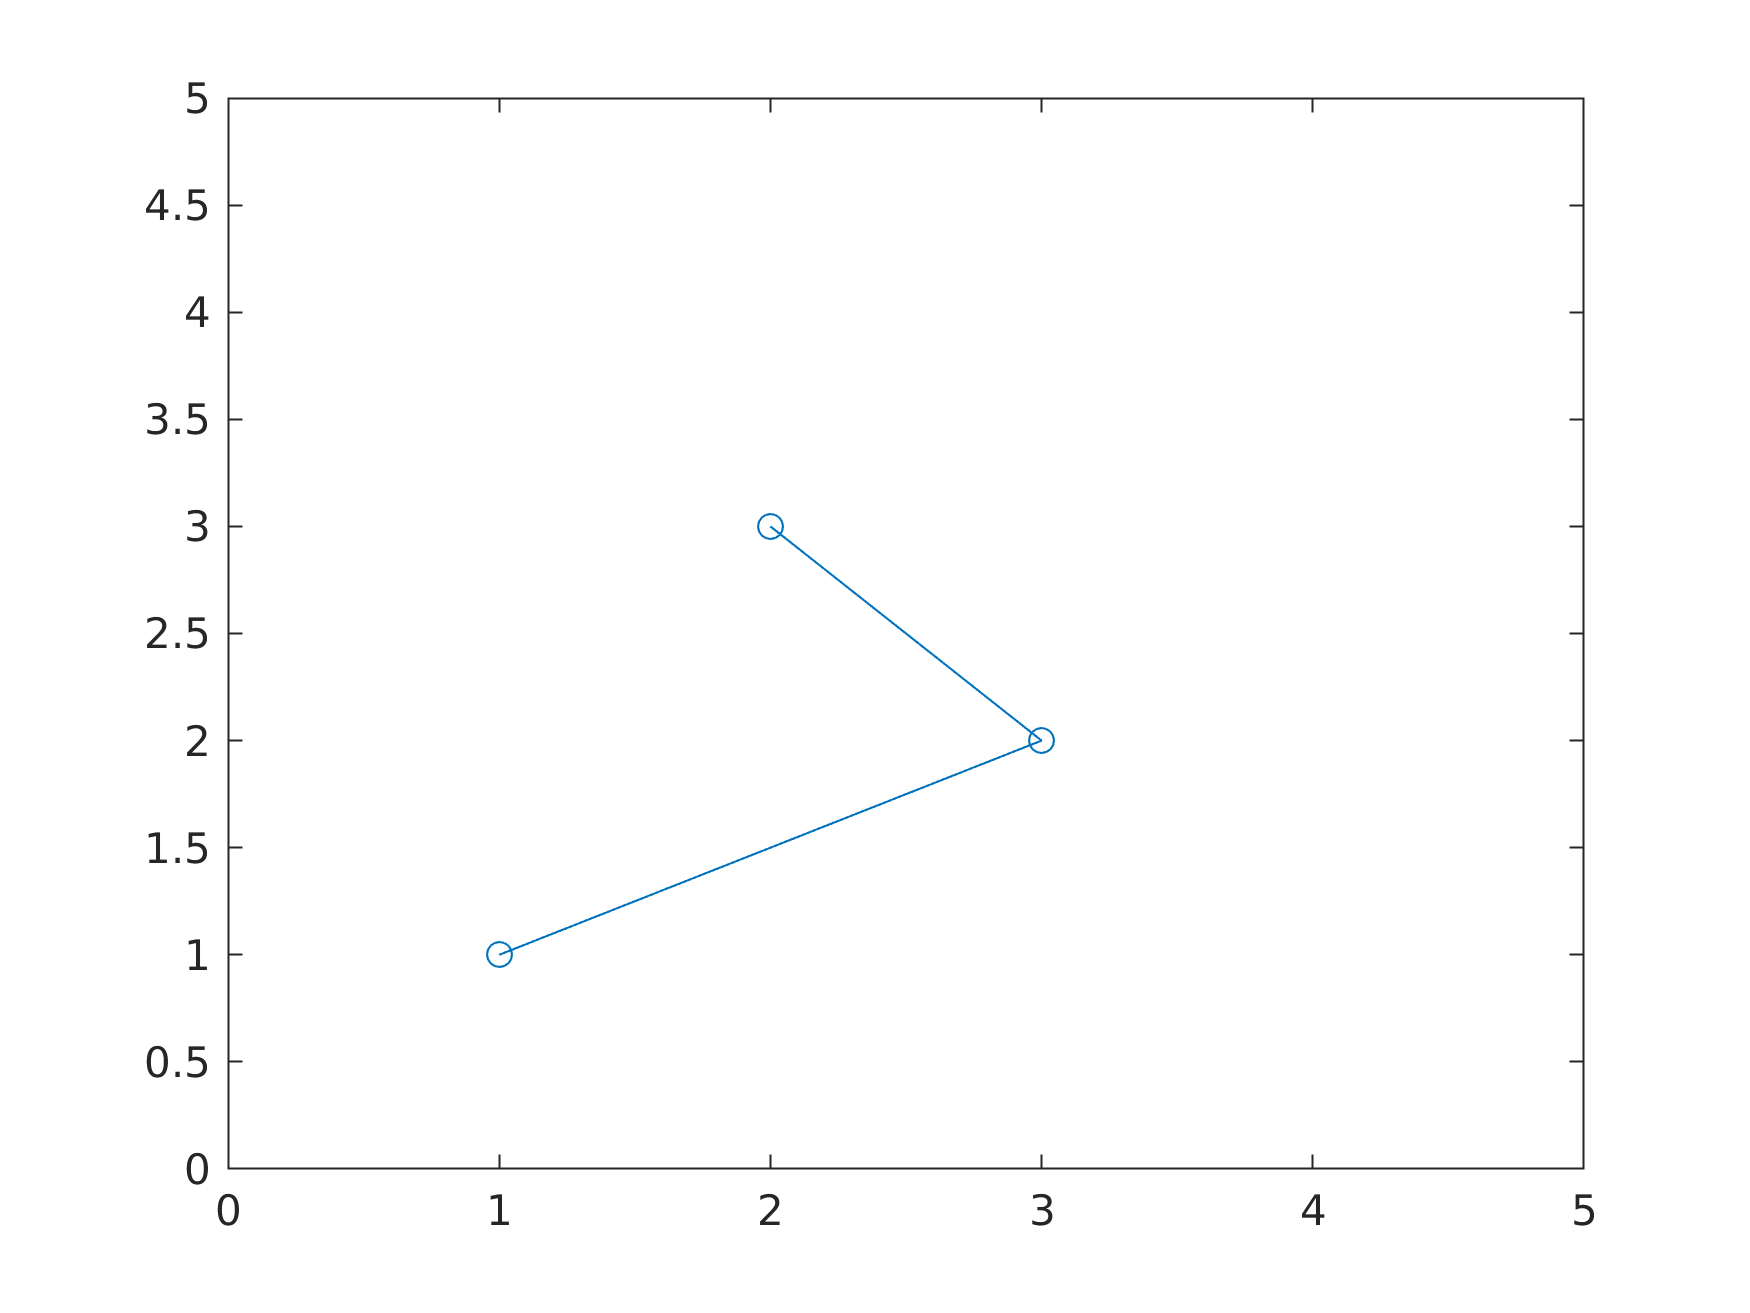
\includegraphics[width=8cm]{pic/plotting/basic_plotting_010.png}
\begin{hint}
The commands \verb!plot!, \verb!xlim! and \verb!ylim! can be useful.
\end{hint}
\begin{sol}
A solution is:
\begin{verbatim}
figure(1);
clf;
x = [1, 3, 2];
y = [1, 2, 3];
plot(x, y, '-o');
xlim([0, 5]);
ylim([0, 5]);
\end{verbatim}
\end{sol}
\end{ex}

\begin{ex}
Find a root of the function $f(x) = e^{-x} - x$.
\begin{hint}
The command \verb!fzero! can be useful.
\end{hint}
\begin{sol}
A solution is:
\begin{verbatim}
fh = @(x) exp(-x) - x
root1 = fzero(fh, 1)
\end{verbatim}
\end{sol}
\end{ex}

\begin{ex}
Find the minimum of the function $f(x) = e^x - 2x$.
\begin{hint}
The command \verb!fminsearch! can be useful.
\end{hint}
\begin{sol}
A solution is:
\begin{verbatim}
fh = @(x) -2x + exp(x);
fminsearch(fh, 1)
\end{verbatim}
\end{sol}
\end{ex}




\begin{ex}
Plot the functions $f(x) = e^x$ and $g(x) = 4x$ over the interval $x \in [-1, 3]$.
\begin{hint}
Define two function handles, one to each function.
Use the functions \verb!linspace!, \verb!hold on!, \verb!plot! and \verb!figure!.
\end{hint}
\begin{sol}
A solution is:
\begin{verbatim}
fh = @(x) exp(x);
gh = @(x) 4*x;
x = linspace(-1, 3);
figure(1);
clf;
hold on;
plot(x, fh(x));
plot(x, gh(x))
\end{verbatim}
\end{sol}
\end{ex}


\begin{ex}
Download the file \verb!test.csv! from this 
\href{https://raw.githubusercontent.com/henrikmidtiby/matlab-notes/master/code/loading_data/test.csv}{link}.
Load the data into matlab and plot the data.
Use the first column as $x$ values and the second column
as $y$ values.
\begin{hint}
\end{hint}
\begin{sol}
A solution is:
\begin{lstlisting}
% Download the datafile, this could also be done
% through the web browser.
url = 'https://raw.githubusercontent.com/henrikmidtiby/matlab-notes/master/code/loading_data/test.csv';
filename = 'test.csv';
outfilename = websave(filename, url);

% Load the data into matlab
data = dlmread(filename);
figure(1);
hold off;
% Plot data in column 1 (the x values) against the 
% data in column 2 (the y values).
%
plot(data(:, 1), data(:, 2));
\end{lstlisting}
\end{sol}
\end{ex}

\begin{ex}
Make the figure inserted below. Pay attention to the axes labels and the width of the plotted line. The visualized function is $f(x) = x^2 - x$. \par
\noindent
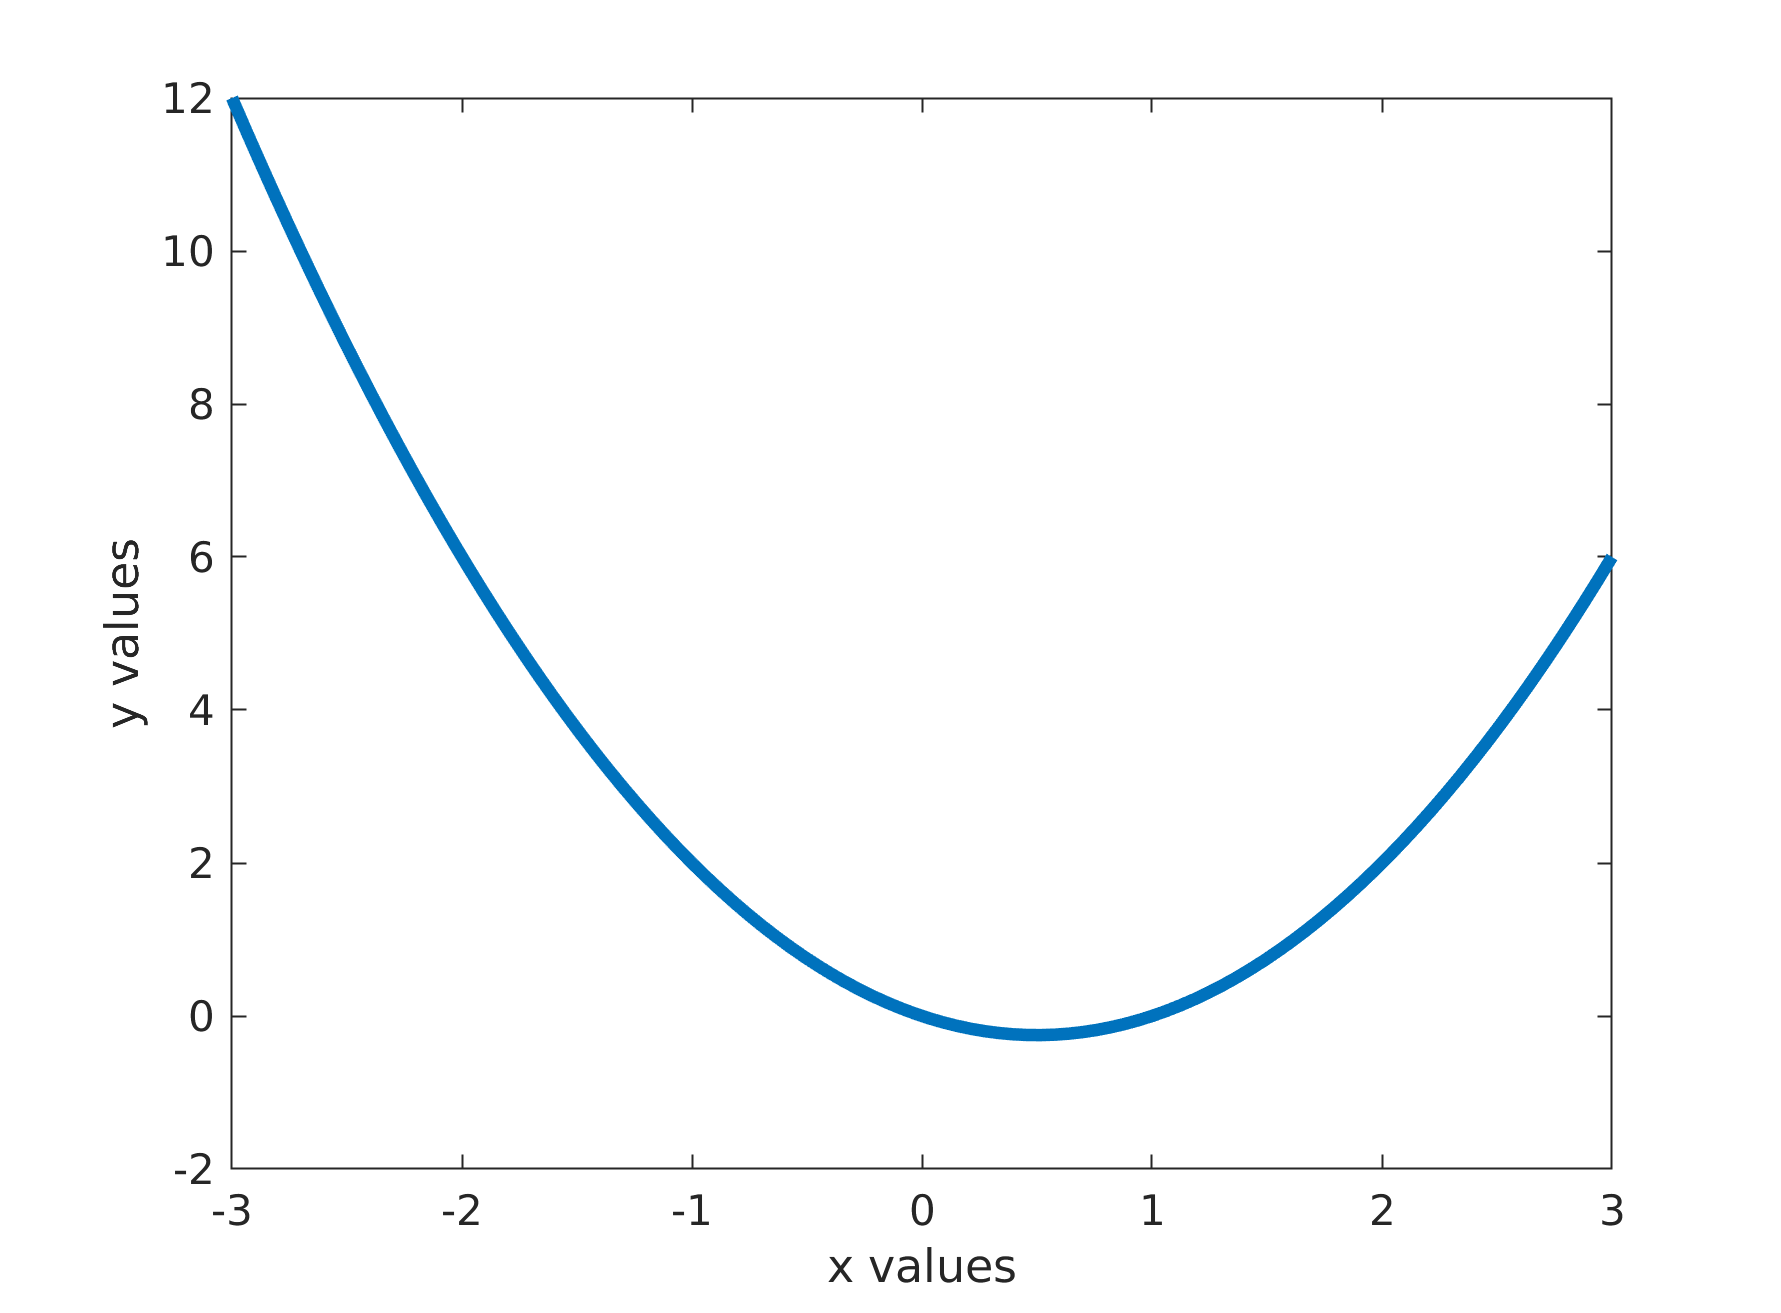
\includegraphics[width=8cm]{pic/plotting/basic_plotting_020.png}
\begin{hint}
The commands \verb!plot!, \verb!xlabel! and \verb!ylabel! can be useful.
\end{hint}
\begin{sol}
A solution is:
\begin{verbatim}
figure(1);
clf;
fh = @(x) -x + x.^2;
x = linspace(-3, 3);
plot(x, fh(x), 'LineWidth', 3);
xlabel('x values');
ylabel('y values');
\end{verbatim}
\end{sol}
\end{ex}


\begin{ex}
Find two numerical solutions to the equation
\[
e^{x} = 4x
\]
\begin{hint}
Write the equation on the form $f(x) = 0$ (collect all elements on the left hand side).
The command \verb!fzero! can be useful.
\end{hint}
\begin{sol}
A solution is:
\begin{verbatim}
% Plot functions (left hand side and right hand side 
% of the equation).
f = @(x) exp(x);
g = @(x) 4*x;
x = linspace(0, 2.5);
figure(1);
hold off;
plot(x, f(x));
hold on;
plot(x, g(x));

% Locate solutions / zeros
difference = @(x) f(x) - g(x);
root1 = fzero(difference, 0.3)
root2 = fzero(difference, 2.1)
\end{verbatim}
\end{sol}
\end{ex}



\begin{ex}
Solve the set of linear equations
\begin{align*}
1	& = 5x + 2y	\\
0	& = -x + y + 3z + 2v	\\
-10 	& = x + 3y - 4z + v	\\
0	& = -2x + 3z - 2v 
\end{align*}
\begin{hint}
Write the system of equations on matrix form $A \cdot \vec{x} = \vec{b}$.
\end{hint}
\begin{sol}
A solution is:
\begin{verbatim}
A = [5, 2, 0, 0; -1, 1, 3, 2; 1, 3, -4, 1; -2, 0, 3, -2];
b = [1; 0; -10; 0];
x = linsolve(A, b)
A * x
\end{verbatim}
\end{sol}
\end{ex}



\begin{ex}
Enter\label{exPlotDataToFitLinearModelTo}
the following values for $x$ and $y$ and plot the points.
Then describe the trend you are observing in the data.
\begin{verbatim}
x = [1, 2, 3, 5];
y = [4, 3, 2, 1];
\end{verbatim}
\begin{hint}
Use the \verb!plot! method.
\end{hint}
\begin{sol}
A solution is:
\begin{verbatim}
x = [1, 2, 3, 5];
y = [4, 3, 2, 1];
figure(1);
clf;
plot(x, y, 'o');
\end{verbatim}
From the plot I see that the $y$ values decreases as the $x$ values increases.
\end{sol}
\end{ex}

\begin{ex}
This\label{exPlotDataToFitLinearModelTo2}
exercise is a continuation of exercise \ref{exPlotDataToFitLinearModelTo}.\\
Implement a linear model $y = a \cdot x + b$ in matlab. 
The linear model should be defined like below, where P is a vector containing the 
model parameters $a$ and $b$.
\begin{verbatim}
model = @(x, P) <fill in stuff here>;
\end{verbatim}
\begin{hint}
The output of the model should match the output below.
\begin{verbatim}
>> model([1, 2, 3, 5], [-1, 5])
ans =
     4     3     2     0
\end{verbatim}
\end{hint}
\begin{sol}
A solution is:
\begin{verbatim}
model = @(x, P) P(1) * x + P(2);
\end{verbatim}
\end{sol}
\end{ex}

\begin{ex}
This \label{exPlotDataToFitLinearModelTo3}
exercise is a continuation of exercise \ref{exPlotDataToFitLinearModelTo2}.\\
Implement a method that calculates the squared error
between the model and observations.
\[
\text{squared error} = \sum_i \left(y_i - \text{model}(x_i)\right)^2
\]
Assume that the $x$ and $y$ values are saved in the variables 
\verb!x! and \verb!y! respectively.
\begin{verbatim}
model_error = @(P) <fill in stuff here>;
\end{verbatim}
\begin{hint}
The \verb!sum! function is helpful.
\end{hint}
\begin{sol}
A solution is:
\begin{verbatim}
>> x = [1, 2, 3, 5];
>> y = [4, 3, 2, 1];
>> model = @(x, P) P(1) * x + P(2);
>> model_error = @(P) sum((y - model(x, P)).^2);
>> squared_error = model_error([-1.2, 5])
squared_error =
    4.5600
\end{verbatim}
\end{sol}
\end{ex}

\begin{ex}
This exercise is a continuation of exercise \ref{exPlotDataToFitLinearModelTo3}. \\
Minimize the squared error, defined in exercise \ref{exPlotDataToFitLinearModelTo3} 
and then plot the model with the 
found parameter values along with the original data.
\begin{hint}
You can try to minimize the function manually by calling it with different 
parameters and then adjust the parameters so that the function value
is reduced. It could look like this.
\begin{lstlisting}
>> squared_error = model_error([-1.2, 5])
squared_error = 4.5600
>> squared_error = model_error([-1.2, 4.5])
squared_error = 8.7600
>> squared_error = model_error([-1.2, 5.5])
squared_error = 2.3600
>> squared_error = model_error([-1.25, 5.5])
squared_error = 3.1875
>> squared_error = model_error([-1.15, 5.5])
squared_error = 1.7275
\end{lstlisting}


The \verb!fminsearch! function is helpful, it should converge to 
the proper solution independent of the initial guess.
The solution contains the following values $-0.7429$ and $4.5429$.
\end{hint}
\begin{sol}
A solution is:
\begin{verbatim}
x = [1, 2, 3, 5];
y = [4, 3, 2, 1];
model = @(x, P) P(1) * x + P(2);
model_error = @(P) sum((y - model(x, P)).^2);
P = fminsearch(model_error, [4, 2])

xvals = linspace(0, 6);
figure(1);
clf;
hold on;
plot(x, y, 'o');
plot(xvals, model(xvals, P));
\end{verbatim}
\end{sol}
\end{ex}



\begin{ex}
Plot the three functions given below in the same plot.
\[
f(x) = \frac{1}{x + 1} \qquad \qquad g(x) = \frac{1}{x + 3} \qquad \qquad h(x) = \frac{1}{(x + 1)(x + 3)}
\]
Do the functions have something in common?
\begin{hint}
Look at the discontinuities of the functions. Where are they placed?
\end{hint}
\begin{sol}
A solution is:
\begin{verbatim}
fh = @(x) 1 ./ (x + 1);
gh = @(x) 1 ./ (x + 3);
hh = @(x) 1 ./ ((x + 1) .* (x + 3));
x = linspace(-5, 1, 1000);
figure(1);
clf; 
hold on;
plot(x, fh(x));
plot(x, gh(x));
plot(x, hh(x));
ylim([-4, 4]);
\end{verbatim}
\end{sol}
\end{ex}

\begin{ex}
Given the three functions below:
\[
f(x) = \frac{1}{x + 1} \qquad \qquad g(x) = \frac{1}{x + 3} \qquad \qquad h(x) = \frac{1}{(x + 1)(x + 3)}
\]
Plot $h(x)$ and a linear combination of $f(x)$ and $g(x)$ in the same plot.
Adjust the coefficients of $f(x)$ and $g(x)$, so that the two plotted functions 
becomes as similar as possible.
\begin{hint}
An example of a linear combination of $f(x)$ and $g(x)$ is
\[
2 \cdot f(x) + 3 \cdot g(x)
\]
\end{hint}
\begin{sol}
A solution is:
\begin{verbatim}
fh = @(x) 1 ./ (x + 1);
gh = @(x) 1 ./ (x + 3);
hh = @(x) 1 ./ ((x + 1) .* (x + 3));
figure(2);
clf; 
hold on;
plot(x, 0.5*fh(x) - 0.5*gh(x));
plot(x, hh(x), 'LineStyle', '- -', 'LineWidth', 3);
ylim([-4, 4]);
\end{verbatim}
\end{sol}
\end{ex}



\begin{ex}
Use the debugger to examine the \verb!binary_log! function.
\begin{enumerate}
\item Open the file \href{https://raw.githubusercontent.com/henrikmidtiby/matlab-notes/master/code/debugger_example_binary_log/binary_log.m}{binary.log}
\item	Insert a \verb!fprintf! statement in line 3, that prints the input arguments given to the function.
\item	Insert a breakpoint (red circle next to the line numbers) at the start of the function "\verb!binary_log!".
\item	Call the function as "\verb!binary_log(8)!" and step through the method using the debugger.
\item	Insert a comment in the function that explains what the while loop in line 6--9 is doing.
\item	Call the function as "\verb!binary_log(0.25)!" and step through the method using the debugger.
\item	Insert a comment in the function that explains what the while loop in line 11--14 is doing.
\end{enumerate}
\begin{hint}
Log rules to be aware of
\[
\log_2(2 \cdot a) = 1 + \log_2(a) \\
\log_2(a / 2) = -1 + \log_2(a)
\]
\end{hint}
\begin{sol}
Lines 6--9 applies the rule $\log_2(2 \cdot a) = 1 + \log_2(a)$ until $a$ is less than 2.

Lines 11--14 applies the rule $\log_2(a / 2) = -1 + \log_2(a)$ until $a$ is greater than or equal to 1.
\end{sol}
\end{ex}
 
% !TeX encoding = UTF-8
% !TeX program = pdfLaTeX
% !TeX root = matlab-exercises-emaip.tex
% !TeX spellcheck = en_GB
\section{Numerical integration}
\SetExerciseDirectory{08_numerical_integration}

\subsection{Trapezoidal rule}
It is not always possible to evaluate the definite integral
\[
\int_a^b f(x) \, dx
\]
as it can be difficult or even impossible to determine the 
anti--derivative $F(x)$.

The value of the definite integral can however be estimated
using numerical methods.
The Trapezoidal rule is one approach for estimating the 
numerical value of the integral, the Trapezoidal rule 
is based on the approximation:
\[
\int_a^b f(x) \, dx \simeq (b - a) \cdot \frac{f(a) + f(b)}{2}
\]

The error of the approximation depends on the function that 
is being integrated $f(x)$ and the length of the integration 
interval.
To reduce the error, the range of the integral can be divided 
into two and then the approximation is applied to each interval.
\begin{align*}
\int_a^b f(x) \, dx 
& = \int_a^c f(x) \, dx + \int_c^b f(x) \, dx \\
& \simeq (c - a) \cdot \frac{f(a) + f(c)}{2} + (b - c) \cdot \frac{f(c) + f(b)}{2}
\end{align*}


\begin{ex}
Explain how the Trapezoidal rule works.
\[
\int_a^b f(x) \, dx \simeq (b - a) \cdot \frac{f(a) + f(b)}{2}
\]
\begin{hint}
Draw a function and the area below the function over the r
range of integration.
Can you recognize the values $(b - a)$ and $\frac{f(a) + f(b)}{2}$
in the figure?
\end{hint}
\begin{sol}
No solution provided yet.
\end{sol}
\end{ex}

\begin{ex}
Plot the function 
\[
f(x) = e^{-x} \cdot \sin(x)
\]
over the range $x \in [0, 5]$.
\begin{hint}
Define a function handle.
Make a list of x values that covers the range.
Apply the function handle to the x values.
Plot the calculated function values against the x values.
\end{hint}
\begin{sol}
A solution is:
\begin{lstlisting}
figure(1);
f = @(x) exp(-x) .* sin(x);
x = linspace(0, 5);
plot(x, f(x));
\end{lstlisting}
\end{sol}
\end{ex}


\begin{ex}[Reference value]\label{exTrapezRuleReference}%
Evaluate the integral below numerically using the \verb!integral! function.
\[
\int_0^5 e^{-x} \cdot \sin(x) \, dx
\]
\begin{hint}
The two first significant digits are 0.50.
\end{hint}
\begin{sol}
A solution is:
\begin{verbatim}
fh = @(x) exp(-x) .* sin(x);
integral(fh, 0, 5)
\end{verbatim}
\end{sol}
\end{ex}

\begin{ex}[Trapezoidal rule example]\label{exTrapezRule}%
Create a list of 10 evenly spaced $x$--values from 
0 to 5, these values will be called $x_i$.
Evaluate the function 
\[
f(x) = e^{-x} \cdot \sin(x)
\]
at these $x$--values and save these values in 
a list called $y_i$.
Then calculate the sum
\[
\sum_{i = 1}^{9} \frac{y_i + y_{i + 1}}{2} \cdot (x_{i + 1} - x_i)
\]
\begin{hint}
Use \verb!linspace! to generate a list of x-values.
\end{hint}
\begin{sol}
A solution based on a for loop is
\begin{lstlisting}
nvals = 10;
x = linspace(0, 5, nvals);

fh = @(x) exp(-x) .* sin(x);
fx = fh(x);

value = 0;
for k = 1:(nvals - 1)
    avg_height = 0.5*(fx(k) + fx(k + 1));
    dx = x(k + 1) - x(k);
    value = value + avg_height * dx;
end
\end{lstlisting}

A more compact solution based on vectorization
is 
\begin{lstlisting}
nvals = 10;
x = linspace(0, 5, nvals);

fh = @(x) exp(-x) .* sin(x);
fx = fh(x);

dx = x(2:end) - x(1:end-1);
avg = 0.5 * (fx(1:end-1) + fx(2:end));
value = dx * avg';
\end{lstlisting}
\end{sol}
\end{ex}

\begin{ex}[Error]%
Calculate the difference between the approximation from 
exercise \ref{exTrapezRule} and the reference values from 
exercise \ref{exTrapezRuleReference}.
\begin{hint}
\end{hint}
\begin{sol}
A solution is:
\begin{lstlisting}
\end{lstlisting}
\end{sol}
\end{ex}


\begin{ex}[Reduced step length]%
Repeat exercise \ref{exTrapezRule}, but use 20 steps instead of 10.
\begin{hint}
Look at the solution to \ref{exTrapezRule} and modify the call to linspace.
\end{hint}
\begin{sol}
\begin{lstlisting}
nvals = 20;
x = linspace(0, 5, nvals);

fh = @(x) exp(-x) .* sin(x);
fx = fh(x);

value = 0;
for k = 1:(nvals - 1)
    avg_height = 0.5*(fx(k) + fx(k + 1));
    dx = x(k + 1) - x(k);
    value = value + avg_height * dx;
end
\end{lstlisting}
\end{sol}
\end{ex}

\begin{ex}[Trapezoidal rule as a function]%
Create a function that uses the Trapezoidal rule to estimate the 
value of a definite integral.
The function must have the signature
\begin{lstlisting}
function res = trapez_rule(fh, x_low, x_high, n_intervals)
\end{lstlisting}
where \verb!fh! is a function handle, 
\verb!x_low! and \verb!x_high! are the integration limits
and \verb!n_intervals! is the number of subintervals 
used for evaluating the integral.
Use the following examples to test the function
\begin{lstlisting}
>> fh = @(x) exp(-x) .* sin(x);
>> trapez_rule(fh, 0, 5, 10)
ans = 0.4770
>> trapez_rule(fh, 0, 5, 20)
ans = 0.4966
>> trapez_rule(fh, 0, 5, 100)
ans = 0.5021
\end{lstlisting}
\begin{hint}
Use your solution from exercise \ref{exTrapezRule} and build a function around it.
\end{hint}
\begin{sol}
A solution is:
\begin{lstlisting}
function res = trapez_rule(fh, x_low, x_high, n_intervals)

x = linspace(x_low, x_high, n_intervals);
fx = fh(x);
res = 0;
for k = 1:(n_intervals - 1)
    avg_height = 0.5*(fx(k) + fx(k + 1));
    dx = x(k + 1) - x(k);
    res = res + avg_height * dx;
end

end
\end{lstlisting}
\end{sol}
\begin{solutionfile}{trapez_rule.m}
function res = trapez_rule(fh, x_low, x_high, n_intervals)

x = linspace(x_low, x_high, n_intervals);
fx = fh(x);
res = 0;
for k = 1:(n_intervals - 1)
    avg_height = 0.5*(fx(k) + fx(k + 1));
    dx = x(k + 1) - x(k);
    res = res + avg_height * dx;
end

end
\end{solutionfile}
\begin{solutionfile}{trapez_rule_test.m}
function tests = trapez_rule_test
    tests = functiontests(localfunctions);
end

%% Test 1: Uniform sampling
function test1(testCase)
    fh = @(x) exp(-x) .* sin(x);
    actual_value =  trapez_rule(fh, 0, 5, 10);
    expected_value = 0.4770;
    testCase.verifyEqual(actual_value, expected_value, ...
        'RelTol', 0.001);
end

%% Test 2: 
function test2(testCase)
    fh = @(x) exp(-x) .* sin(x);
    actual_value =  trapez_rule(fh, 0, 5, 20);
    expected_value = 0.4966;
    testCase.verifyEqual(actual_value, expected_value, ...
        'RelTol', 0.001);
end

\end{solutionfile}
\end{ex}

\begin{ex}
Investigate how the numerical error of the estimate decreases 
as the number of intervals are increased.
Make a table of the used step lengths and the 
associated errors.
To do this you will have to select a function and an 
interval over which the definite integral should be
calculated.
\begin{hint}
Call the \verb!trapez_rule! function with different 
number of steps.
For each call of the function, write the step length
and the error to the console.
\end{hint}
\begin{sol}
A solution is: 
\begin{lstlisting}
fh = @(x) exp(-x) .* sin(x);
xlow = 0;
xhigh = 5;
ref = integral(fh, xlow, xhigh);

for k = 1:10
    steps = 2^k;
    val = trapez_rule(fh, xlow, xhigh, steps);
    fprintf("%8.3f %8.3f\n", (xhigh - xlow) / steps, val - ref);
end
\end{lstlisting}
The error is seen to be proportional to the step length
squared.
\end{sol}
\end{ex}


\begin{ex}
Estimate the values of the integrals
\[
V_1 = \int_1^3 \sin(2x) \, dx \qquad \textrm{and} \qquad
V_2 = \int_2^6 \frac{\sin(x)}{2} \, dx.
\]
How would you expect them to be related?
\begin{hint}
Use the \verb!integral! function.
The substitution rule has been applied to the first
integral and this has generated the second integral.
\end{hint}
\begin{sol}
A solution is
\begin{lstlisting}
fh1 = @(x) sin(2*x);
fh2 = @(x) sin(x) / 2;
integral(fh1, 1, 3)
integral(fh2, 2, 6)
\end{lstlisting}

As the integrals are related to each other 
through the substitution rule, they should have 
the exact same value; which is also confirmed 
using matlab.
\end{sol}
\end{ex}



 
% !TeX encoding = UTF-8
% !TeX program = pdfLaTeX
% !TeX root = matlab-exercises-emaip.tex
% !TeX spellcheck = en_GB
\section{Functions and recap}
\SetExerciseDirectory{09_functions}

\subsection{Plotting and normalizing data}

\begin{ex} \label{exComparingRawDataSets}%
Four datasets with amplitude over time have been 
placed in your git repository in the location
\verb!18_dealing_with_experimental_data/data!.
Plot these four datasets in one figure.
\begin{hint}
Load the datasets one by one at the time using the \verb!dlmread! function.
For each dataset extract the x and y values (first and second column).
Plot the x and y values.
\end{hint}
\begin{sol}
A solution is:
\begin{lstlisting}
data = dlmread('data/dataset_01.csv');
x = data(:, 1);
y = data(:, 2);

figure(1);
clf;
plot(x, y);
hold on;

data = dlmread('data/dataset_02.csv');
x = data(:, 1);
y = data(:, 2);
plot(x, y);

data = dlmread('data/dataset_03.csv');
x = data(:, 1);
y = data(:, 2);
plot(x, y);

data = dlmread('data/dataset_04.csv');
x = data(:, 1);
y = data(:, 2);
plot(x, y);
\end{lstlisting}
\end{sol}
\end{ex}


\begin{ex}
Improve the plotting of the datasets in exercise 
\ref{exComparingRawDataSets} by normalizing the data
in the following way.
In this exercise you will probably have to repeat the plots 
multiple times and locate specific values in the plot using the
\emph{Data Tips} tool in the plot window.

Shift the x values such that the initial value (at $x = 0$) is
at a maximum.
Scale the y values such that the initial value (at $x = 0$) is one.
Then scale the x values such that one full oscillation of the
system has occurred at $x = 1$.
After shifting and scaling the plotted data should 
have local maxima at $x = 0$, $x = 1$, $x = 2$, $x = 3$, \ldots

The purpose of the normalizations is to make it easier to 
compare datasets acquired under different conditions.
\begin{hint}
To shift the x values a fixed value should be subtracted from the x 
value.
To scale the y values it should be divided with a fixed value.
To scale the x values it should be divided with a fixed value.
\end{hint}
\begin{sol}
A solution is:
\begin{lstlisting}
%%
data = dlmread('data/dataset_01.csv');
x = data(:, 1);
y = data(:, 2);
figure(5)
clf;
first_peak = -1.255;
cycle_length = 1.526;
peak_value = 0.87;
plot((x-first_peak) / cycle_length, y / peak_value);
hold on;
%xlim([0, 6]);

%%
data = dlmread('data/dataset_02.csv');
x = data(:, 1);
y = data(:, 2);
figure(5)
first_peak = -1.447;
cycle_length = 2.859 / 2;
peak_value = 1.05;
plot((x-first_peak) / cycle_length, y / peak_value);

%%
data = dlmread('data/dataset_03.csv');
x = data(:, 1);
y = data(:, 2);
figure(5)
first_peak = -0.9429;
cycle_length = 4.552 / 4;
peak_value = 1.25;
plot((x-first_peak) / cycle_length, y / peak_value);

%%
data = dlmread('data/dataset_04.csv');
x = data(:, 1);
y = data(:, 2);
figure(5)
first_peak = -1.892;
cycle_length = 3.243 / 5;
peak_value = 2.3;
plot((x-first_peak) / cycle_length, y / peak_value);
\end{lstlisting}
\end{sol}
\end{ex}



\begin{ex}
\begin{tcolorbox}
This exercise is meant as a challenge, it is much more difficult 
than the standard exercises.
Consider this an optional exercise, you do not have to 
solve it.
\end{tcolorbox}
Locate the file \verb!18_dealing_with_experimental_data/mystery_function.m! and figure out what the function actually does 
(and how).
\begin{hint}
Try to plot information from inside the function.
You an also try to rename the variable names, so they 
become more meaningful.
\end{hint}
\begin{sol}
No solution provided.
\end{sol}
\end{ex}



\subsection{Function handles}

We have earlier worked with functions that take numbers and lists 
as input arguments.
But a function can also take a function handle as input argument.
A function handle is a reference to a specific function. 
In the example below is a reference to the sinus function created 
and later tested.
%
\begin{lstlisting}
>> functionHandle = @sin;
>> functionHandle(0.123)
ans = 0.1227
>> sin(0.123)
ans = 0.1227
\end{lstlisting}
%
A function handle can also be generated without using an existing function as template.
The following syntax lets you create function handles from scratch.
%
\begin{lstlisting}
@(input parameters) code to calculate result
\end{lstlisting}
%
As an example the second order Taylor expansion for $\cos(x)$ 
is used to create a function handle.
\begin{lstlisting}
>> fh = @(x) 1 - 0.5*x.^2;
>> cos([0, 0.1, 0.3])
ans = 1.0000    0.9950    0.9553
>> fh([0, 0.1, 0.3])
ans = 1.0000    0.9950    0.9550
\end{lstlisting}

\begin{ex}
Create a function handle named \emph{sumOfSineAndCosine} for the expression
\begin{align*}
f(x) & = \sin(x) + \cos(x)
\end{align*}
Example usage of the function:
\begin{lstlisting}
>> sumOfSineAndCosine([0, 0.1, 0.2, 0.3, 1])
ans = 1.0000    1.0948    1.1787    1.2509    1.3818
\end{lstlisting}
\begin{hint}
Use the syntax
\begin{lstlisting}
fname = @(x) expression;
\end{lstlisting}
Where \verb!fname! and \verb!expression! should be modified.
\end{hint}
\begin{sol}
To create the function handle, run the code below in the matlab command window.
\begin{lstlisting}
sumOfSineAndCosine = @(x) sin(x) + cos(x);
\end{lstlisting}
\end{sol}
\end{ex}



\begin{ex}
Create a function that takes a function handle and a list as input arguments.
The output should be a list with the same number of elements as the input list.
The values in the output list should be the value returned by the function handle 
when applied to the corresponding element in the input list.
The function signature should be:
\begin{lstlisting}
function res = applyFunctionHandleToList(fh, list)
\end{lstlisting}
Example usage of the function:
\begin{lstlisting}
>> applyFunctionHandleToList(@(x) 1, [1, 3, 9])
ans = 1     1     1
>> applyFunctionHandleToList(@(x) 1-x, [1, 3, 9])
ans = 0    -2    -8
\end{lstlisting}
\begin{hint}
Use a for loop to iterate over the input list.
\end{hint}
\begin{sol}
A solution is:
\begin{lstlisting}
function res = applyFunctionHandleToList(fh, list)

res = list;
for idx = 1:length(list)
	res(idx) = fh(list(idx));
end

end
\end{lstlisting}
\end{sol}
\end{ex}


\subsection{Things from old exam sets}

\begin{ex}
Create a function that calculates the n'th Fibonacci number. The nth
fibonacci number can be calculated using the formula: 
\[
F_n = F_{n-1} + F_{n-2}
\]
with the two base cases $F_0 = 0$ and $F_1 = 1$. The sequence goes like
$0, 1, 1, 2, 3, 5, 8, 13, 21, 34, ...$
\begin{lstlisting}
function res = fib(n)
\end{lstlisting}
Example usage of the function:
\begin{lstlisting}
>> fib(0);
>> fib(0)
ans = 0
>> fib(1)
ans = 1
>> fib(6)
ans = 8
>> fib(17)
ans = 1597
>> fib(29)
ans = 514229
\end{lstlisting}
\begin{hint}
Use one or more if statements to ensure that the two base
cases are handled properly.
Then use the relation
\[
\textrm{fib}(n) = \textrm{fib}(n - 1) + \textrm{fib}(n - 2)
\]
\end{hint}
\begin{sol}
A solution is:
\begin{lstlisting}
function res = fib(n)

if(n < 2)
  res = n;
else
  res = fib(n - 1) + fib(n - 2);
end
end
\end{lstlisting}
\end{sol}
\begin{solutionfile}{fib_test.m}
function tests = fib_test
    tests = functiontests(localfunctions);
end


%% The Fibonacci sequence
% Create a function that calculates the n'th Fibonacci number. The nth
% fibonacci number can be calculated using the formula: 
% F_n = F_{n-1} + F_{n-2}
% with the two base cases F_0 = 0 and F_1 = 1. 
% The sequence goes like 0, 1, 1, 2, 3, 5, 8, 13, 21, 34, ...
% The function should have the signature
% function res = fib(n)

%% Test 1: Identical inputs
function test1(testCase)
    actual_value = fib(0);
    expected_value = 0;
    testCase.verifyEqual(actual_value, expected_value);
end
function test2(testCase)
    actual_value = fib(1);
    expected_value = 1;
    testCase.verifyEqual(actual_value, expected_value);
end
function test3(testCase)
    actual_value = fib(2);
    expected_value = 1;
    testCase.verifyEqual(actual_value, expected_value);
end
function test4(testCase)
    actual_value = fib(6);
    expected_value = 8;
    testCase.verifyEqual(actual_value, expected_value);
end
function test5(testCase)
    actual_value = fib(17);
    expected_value = 1597;
    testCase.verifyEqual(actual_value, expected_value);
end
function test6(testCase)
    actual_value = fib(29);
    expected_value = 514229;
    testCase.verifyEqual(actual_value, expected_value);
end
\end{solutionfile}
\begin{solutionfile}{fib.m}
function res = fib(n)

if(n < 2)
  res = n;
else
  res = fib(n - 1) + fib(n - 2);
end
end
\end{solutionfile}
\end{ex}





% 2020-01-24 Reexam
\begin{ex}
Recreate the figure below:
\begin{center}
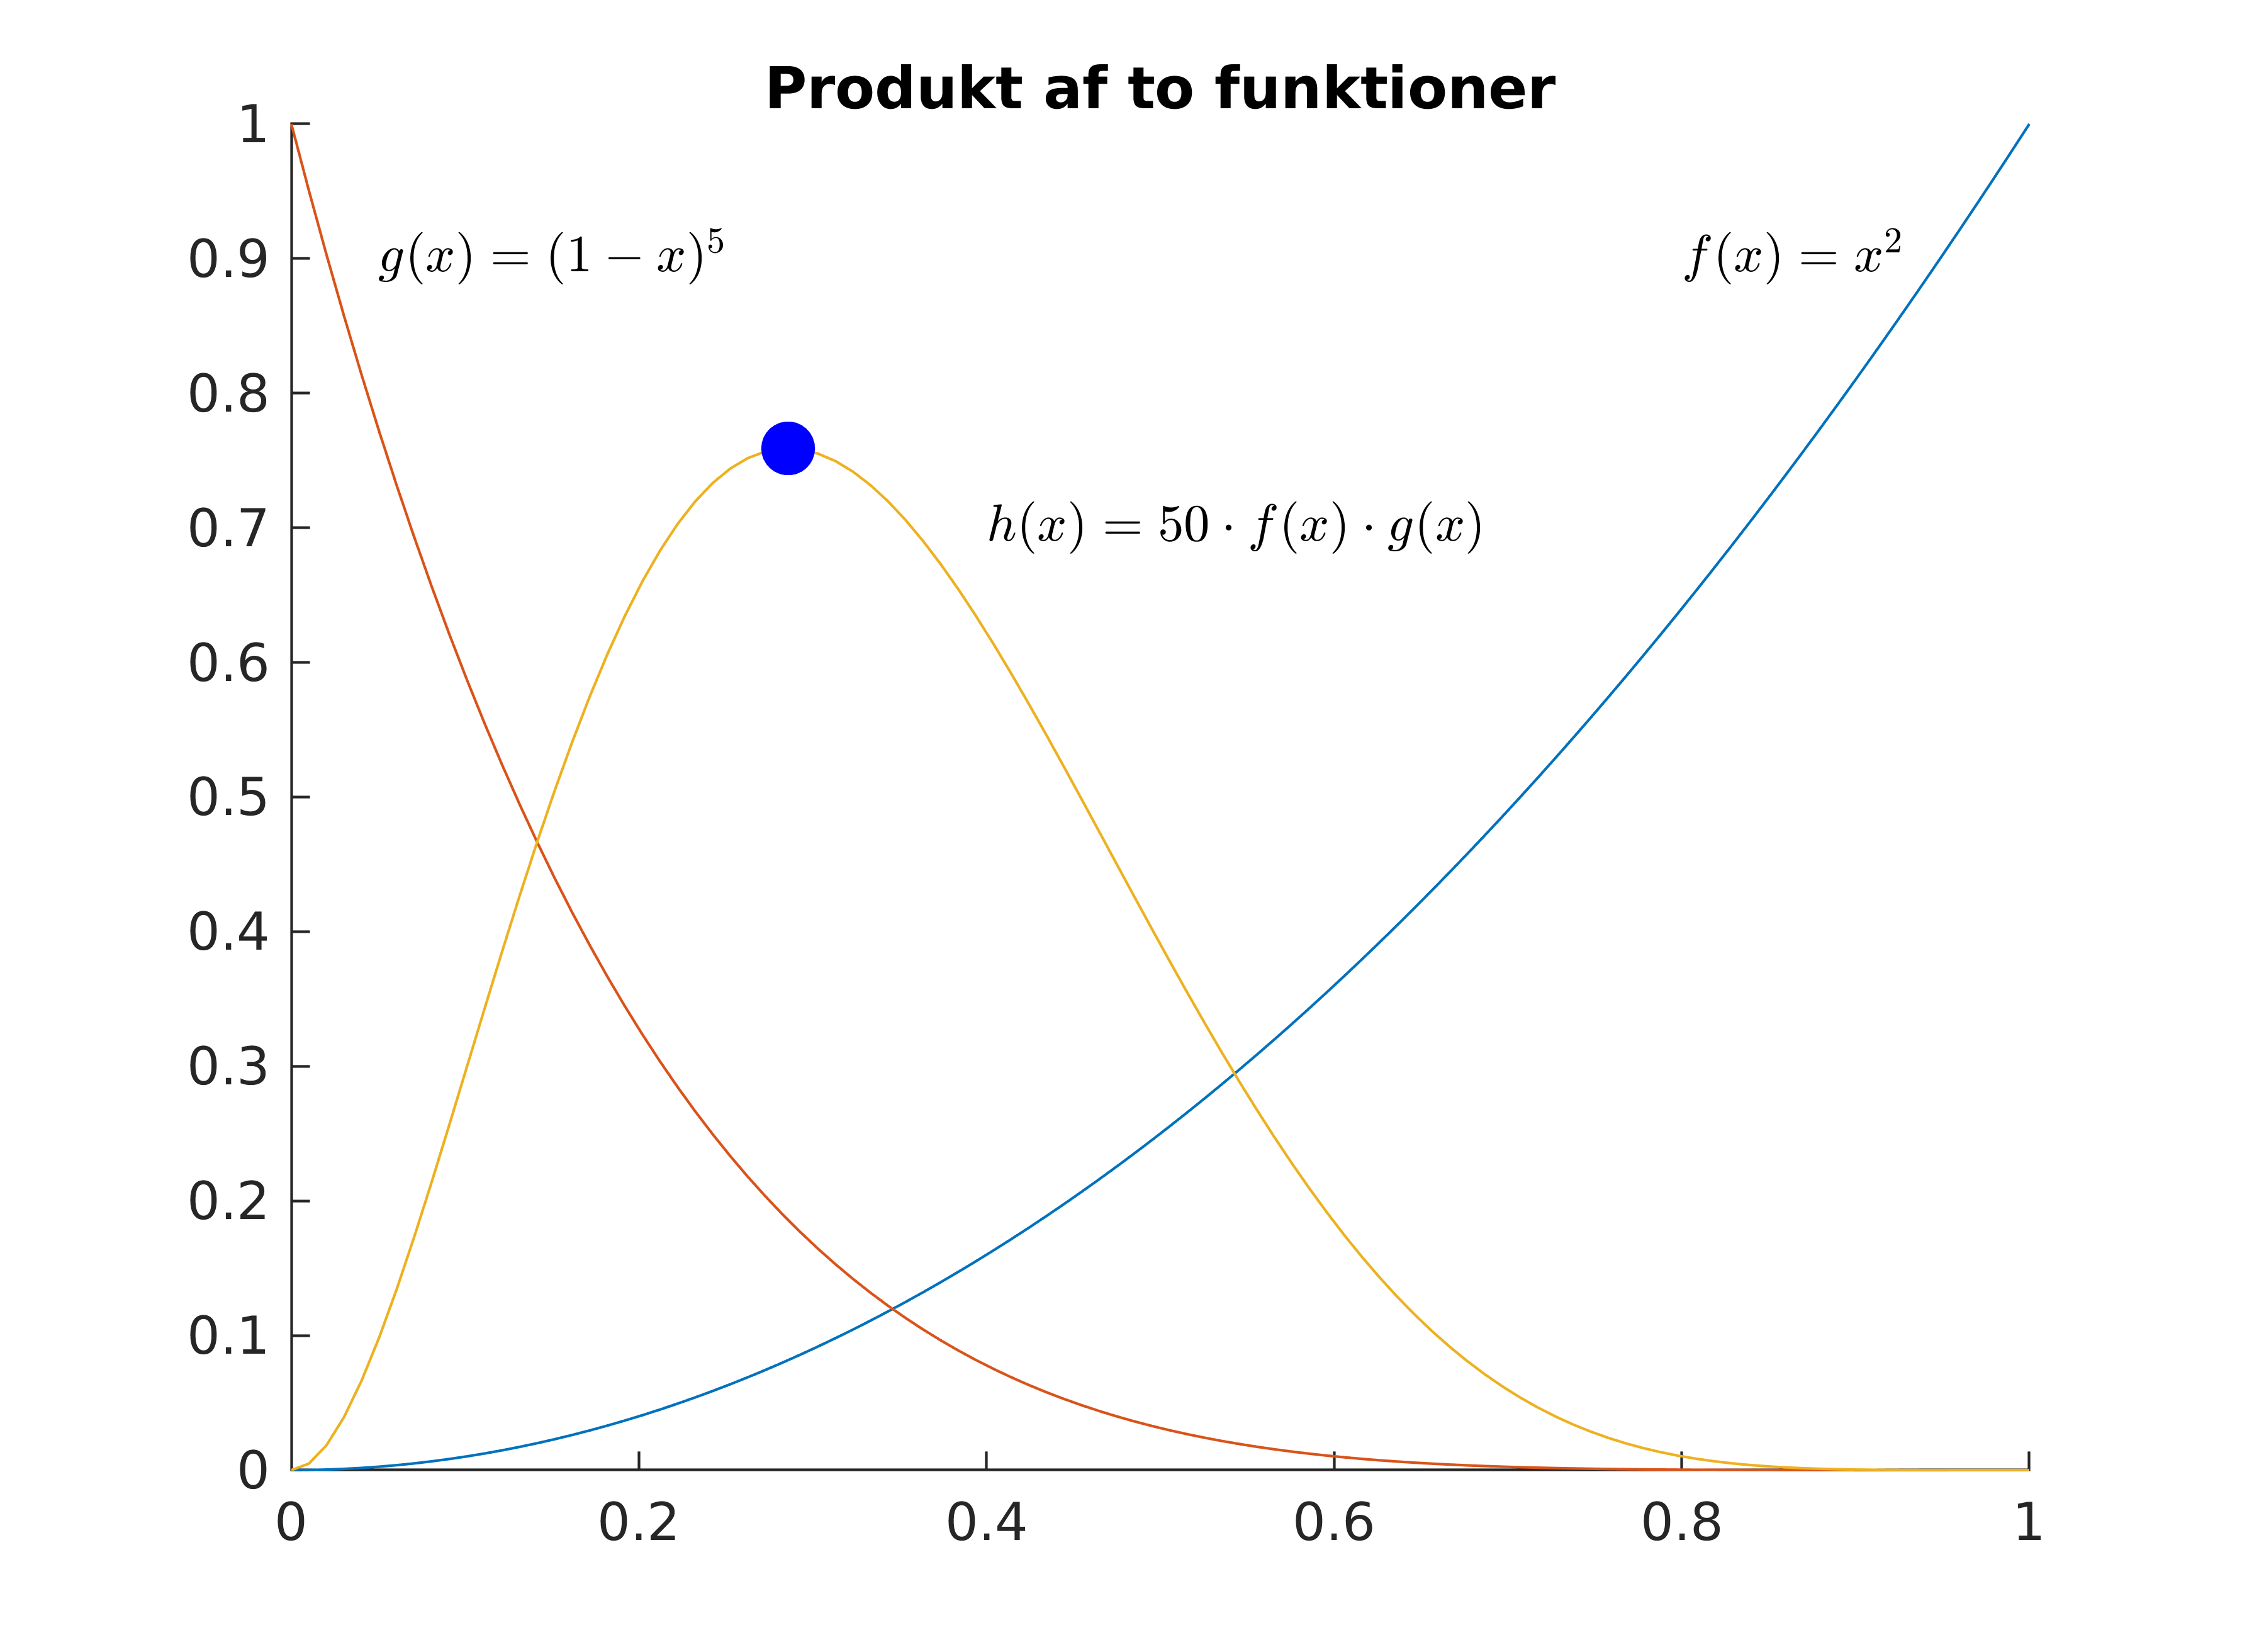
\includegraphics[width=0.7\textwidth]{pic/plotting/product_of_two_functions.png}
\end{center}
\begin{hint}
\end{hint}
\begin{sol}
A solution is:
\begin{lstlisting}
% Exercise 1: Recreate a figure

% Define f(x), g(x) and the range of x values that should be plotted.
fh = @(x) x.^2;
gh = @(x) (1-x).^5;
hh = @(x) 50*fh(x) .* gh(x);
xvals = linspace(0, 1);

% Locate minima of h(x).
h_minima = fminsearch(@(x) -hh(x), 0.2);

% Start a new figure
figure(1);
clf;
hold on;

% Plot functions.
plot(xvals, fh(xvals));
plot(xvals, gh(xvals));
plot(xvals, hh(xvals));

% Indicate locations of roots.
plot(h_minima, hh(h_minima), '.b', 'MarkerSize', 35);

% Add text to plot.
text(0.8, 0.9, "$f(x) = x^2$", ...
    'interpreter', 'latex');
text(0.05, 0.9, "$g(x) = (1-x)^5$", ...
    'interpreter', 'latex');
text(0.4, 0.7, "$h(x) = 50 \cdot f(x) \cdot g(x)$", ...
    'interpreter', 'latex');

% Add title and axis labels.
title("Produkt af to funktioner");
%xlabel('x akse');
%ylabel('y akse');
ylim([0, 1]);

% Write the figure to disk.
print('product_of_two_functions.png', '-dpng', '-r600');
\end{lstlisting}
\end{sol}
\end{ex}







\begin{ex}
Determine the value of the following definite integral:
\begin{align*}
\int_0^1 x^2 \cdot  (1 - x)^5 \; dx
\end{align*}
Then determine the value of $\alpha$, which solves the 
equation below.
\begin{align*}
\frac{1}{2} \cdot \int_0^1 x^2 \cdot  (1 - x)^5 \; dx = \int_0^\alpha x^2 \cdot  (1 - x)^5 \; dx
\end{align*}
\begin{hint}
\end{hint}
\begin{sol}
A solution is:
\begin{lstlisting}
format long

hh = @(x) x.^2 .* (1-x).^5;

val = integral(hh, 0, 1)
integral(hh, 0, 0.3205189672974762) / val

%%
temp = @(x) integral(hh, 0, x) - 0.5 * val;
fzero(temp, 0.5)

format short
\end{lstlisting}
\end{sol}
\end{ex}

\begin{ex}
Create a function that classifies triangles into a set of
types according to their side lengths.
The function should have the signature:
\begin{lstlisting}
function res = triangle_type(a, b, c)
\end{lstlisting}
The input to the function is the length of the 
three sides of the triangle in increasing order ($a \le b \le c$).
The triangle types that should be recognized are:
\begin{description}
\item[impossible] it is not possible to construct a triangle with the given side lengths: $a + b < c$.
\item[equilateral] all sides in the triangle has the same length
\item[obtuse] has an angle above 90 degrees, has the property $a^2 + b^2 < c^2$
\item[right] one of the angles is precisely 90 degrees and the side lengths has the property $a^2 + b^2 = c^2$
\item[acute] all angles are below under 90 grader, the triangle has the property $a^2 + b^2 > c^2$
\end{description}
Use the following examples to test the function
\begin{lstlisting}
>> triangle_type(1, 2, 4)
ans = 'impossible'
>> triangle_type(2, 3, 4)
ans = 'obtuse'
>> triangle_type(3, 4, 5)
ans = 'right'
>> triangle_type(3, 3, 3)
ans = 'equilateral'
>> triangle_type(3, 3, 4);
>> triangle_type(3, 3, 4)
ans = 'acute'\end{lstlisting}
\begin{hint}
\end{hint}
\begin{sol}
A solution is:
\begin{lstlisting}
\end{lstlisting}
\begin{solutionfile}{triangle_type.m}
function res = triangle_type(a, b, c)
% Assume a < b < c

if(c - a - b > 0)
    res = 'impossible';
else
    if(abs(a - c) < 0.0000001)
        res = 'equilateral';
    else
        value = a^2 + b^2 - c^2;
        if(value > 0)
            res = 'acute';
        else
            if(value < 0)
                res = 'obtuse';
            else
                res = 'right';
            end
        end
    end
end
end
\end{solutionfile}
\end{sol}
\end{ex}


\pagebreak[4]
\subsection{Multiple plots in one}
\label{ssecMultiplePlotsInOne}

It is possible to put multiple plots 
next to each other in a single plot in matlab.
This can be done using the subplot command.
The plot shown below
was generated by the code next to it.
\begin{multicols}{2}
\begin{lstlisting}
x = linspace(-5, 5);

figure(1);
clf;

subplot(2, 1, 1);
plot(x, sin(x));
title('Sin(x)');
ylim([-1.5, 1.5]);

subplot(2, 1, 2);
plot(x, x);
hold on;
plot(x, sin(x));
title('Taylor 1');
ylim([-1.5, 1.5]);
\end{lstlisting}
\columnbreak
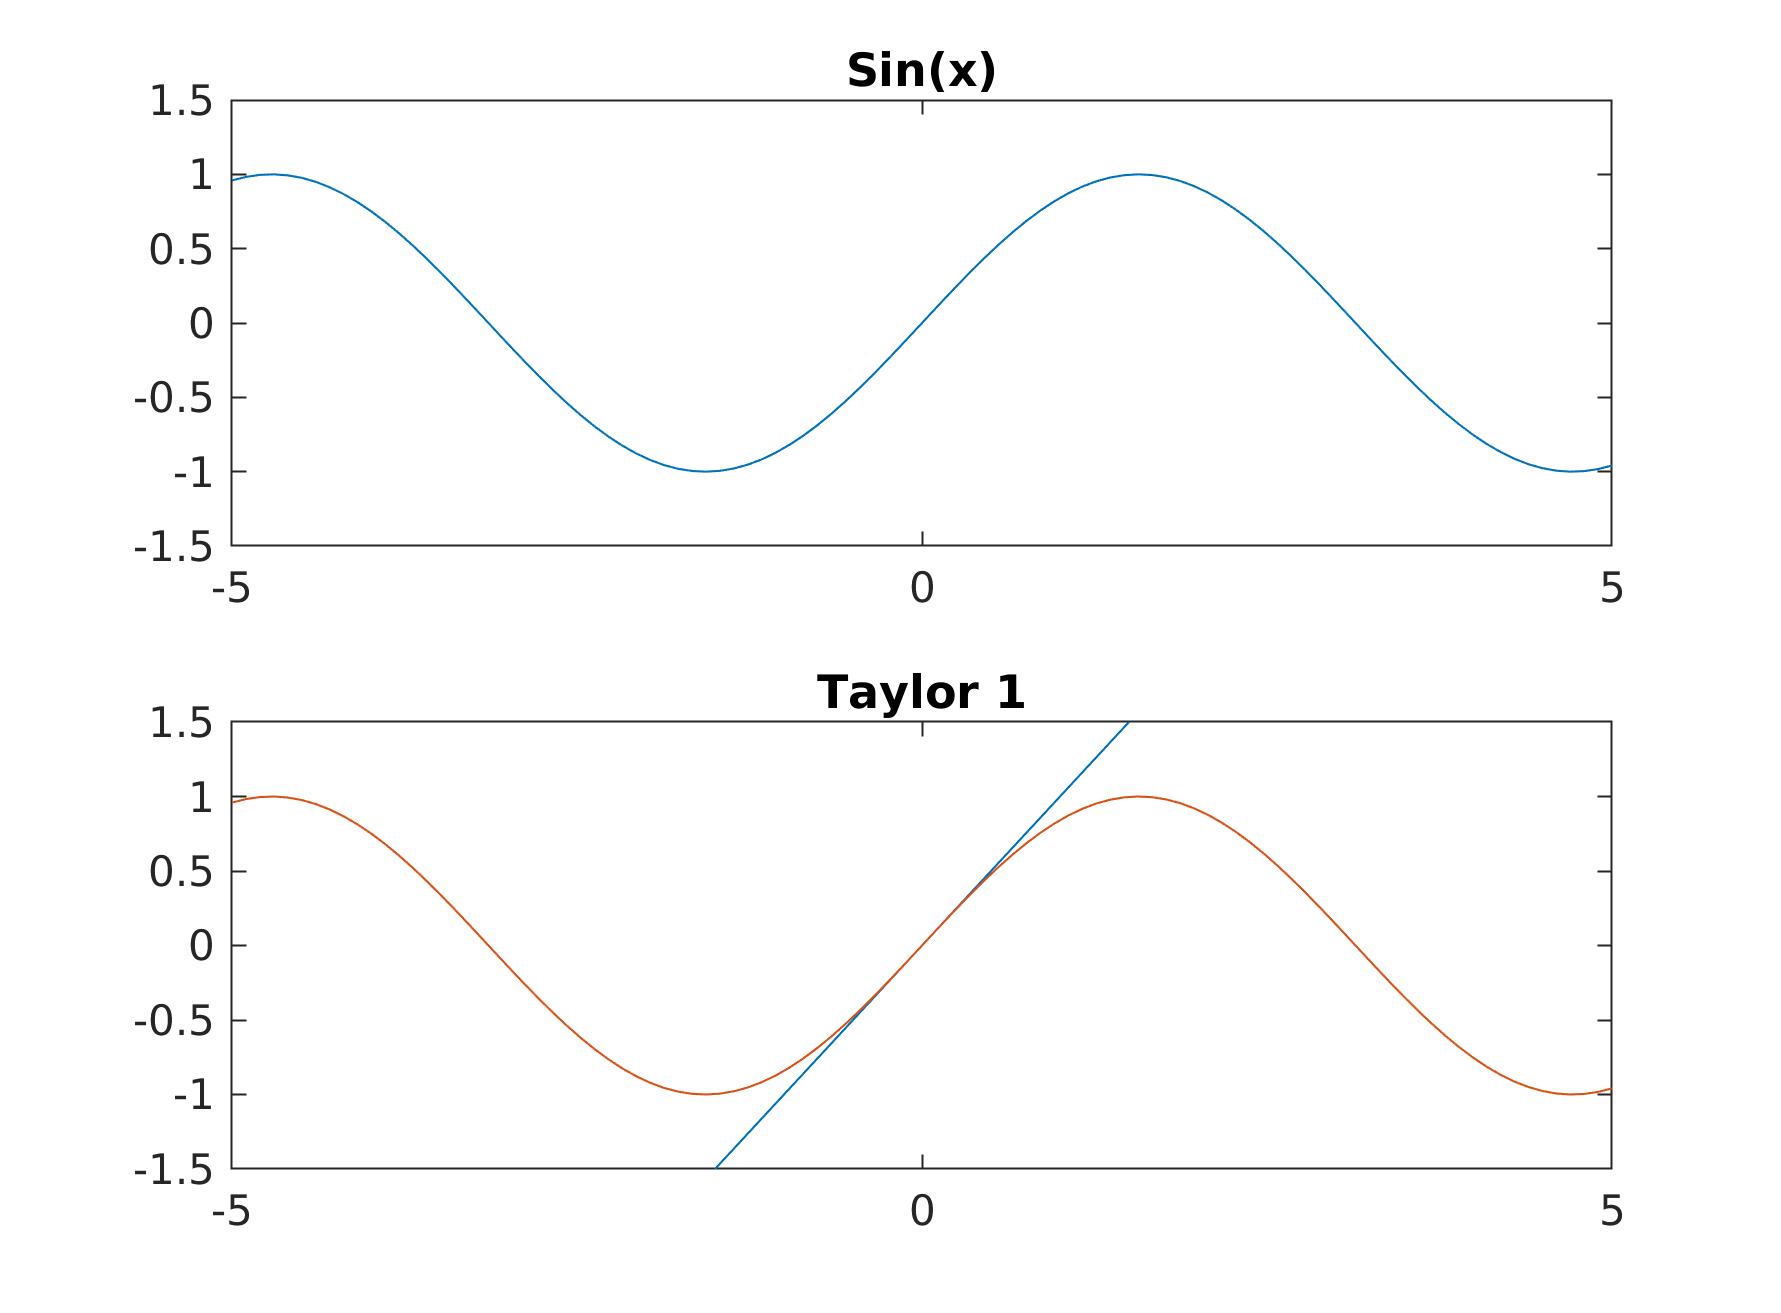
\includegraphics[width=\linewidth]{pic/plotting/subplot_example_1.png}
\end{multicols}

The three input parameters to the \verb!subplot! command
are as follows: 
\begin{itemize}
\item		the number of rows of subplots in the plot
\item		the number of columns of subplots in the plot
\item		a number indicating the subplot in which the following plot commands will operate.
\end{itemize}
The subplots are numbered row wise, so in a subplot 
with two rows and three columns, the subplot numbers will be
distributed as follows:
\begin{align*}
\begin{matrix}
1 & 2 & 3 \\
4 & 5 & 6
\end{matrix}
\end{align*}




\begin{ex}
Recreate the following plot: 
\begin{center}
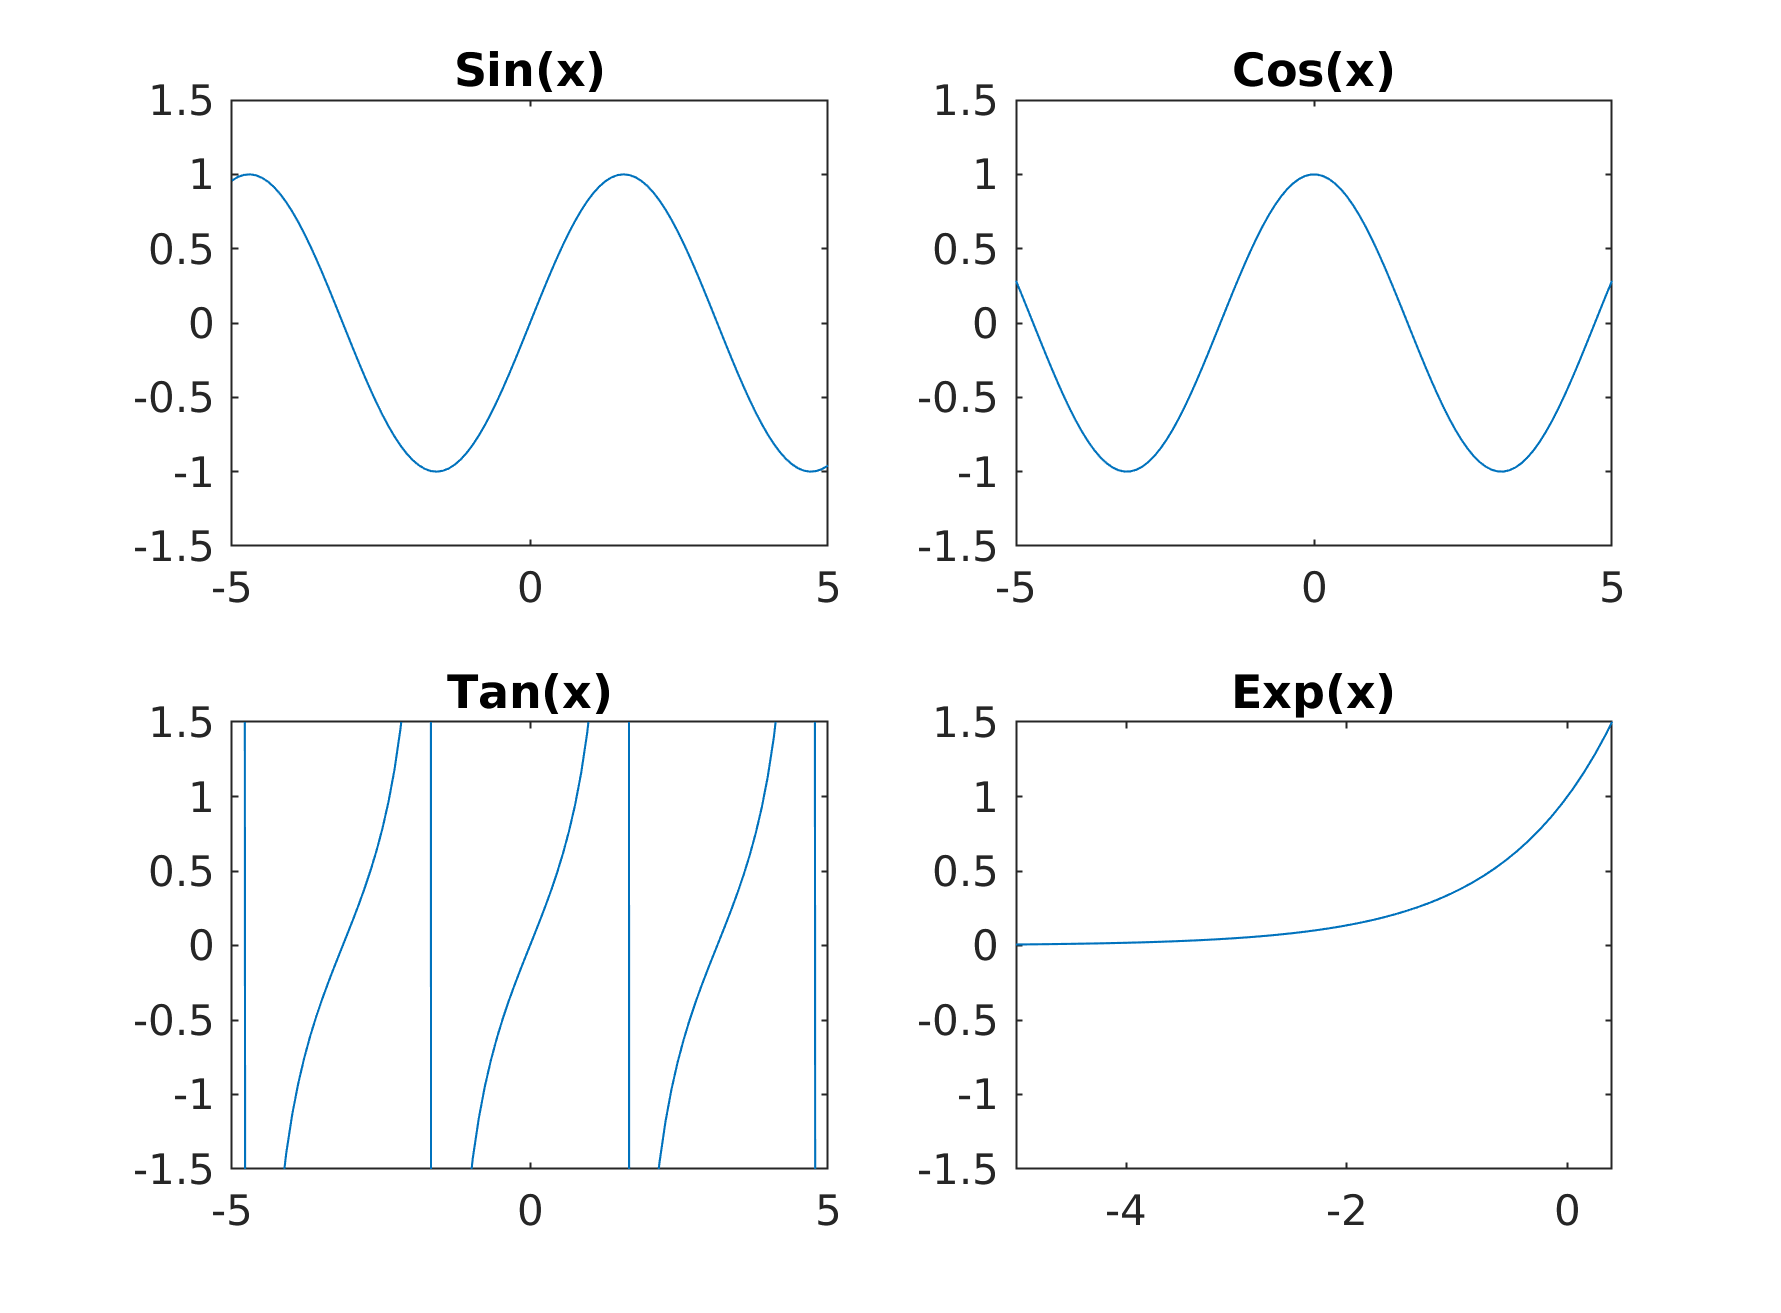
\includegraphics[width=9cm]{pic/plotting/subplot_exercise_1.png}
\end{center}
\begin{hint}
\end{hint}
\begin{sol}
A solution is:
\begin{lstlisting}
\end{lstlisting}
\end{sol}
\end{ex}
 
% !TeX encoding = UTF-8
% !TeX program = pdfLaTeX
% !TeX root = matlab-exercises-emaip.tex
% !TeX spellcheck = en_GB
\section{Numerical solutions of differential equations}
\SetExerciseDirectory{10_numerical_differential_equations}





\subsection{Numerical solutions of differential equations}

Initial value problems, where a differential equation and 
an initial condition are given, can be solved using numeric methods.
Here it is assumed that the differential equation can be 
written in the form
\begin{align}
\label{eqnDiffEquationForm}
\frac{dy}{dx} = f(x, y(x))
\end{align}

\subsubsection{Euler's method}
One of the methods that can be used to approximate the solution
to the initial value problem is Euler's method.
Euler's method is based on the approximation
\begin{align*}
\frac{dy}{dx} = \frac{y(x + h) - y(x)}{h}
\end{align*}
with a step size $h$.
Combined with the differential equation
\eqref{eqnDiffEquationForm}, this lead to the expression
\begin{align*}
\frac{y(x + h) - y(x)}{h} = f(x, y(x))
\end{align*}
by rearranging we obtain
\begin{align*}
y(x + h) = y(x) + h \cdot f(x, y(x))
\end{align*}

Lets look at the initial value problem given below
\begin{align*}
\frac{dy}{dx} = f(x, y(x)) = y	&& y(0) = 1
\end{align*}
To approximate the value of $y(1)$, we can use a single
step with $h = 1$, or multiple steps with a smaller step
length.
First lets examine $h = 1$.
\begin{align*}
y(0) & = 1 \\
y(1) & = y(0) + 1 \cdot f(0, y(0)) \\
& = 1 + 1 \cdot f(0, 1) \\
& = 1 + 1 \cdot 1 \\
& = 2
\end{align*}

Then lets look at $h = 0.5$, now two steps are required to 
estimate the value of $y(1)$.
\begin{align*}
y(0) & = 1 \\
y(0.5) & = y(0) + 0.5 \cdot f(0, y(0)) \\
& = 1 + 0.5 \cdot f(0, 1) \\
& = 1 + 0.5 \cdot 1 \\
& = 1.5 \\
y(1.0) & = y(0.5) + 0.5 \cdot f(0, y(0.5)) \\
& = 1.5 + 0.5 \cdot f(0, 1.5) \\
& = 1 + 0.5 \cdot 1.5 \\
& = 2.25
\end{align*}

When comparing the two approximations for $y(1)$, 
we see that they differ quite much (2 vs. 2.25).
This difference is caused by the approximation error of the method.
The approximation error is reduced when the step length is reduced.


\begin{ex}[Eulers method]%
Implement Euler's method.
The function containing the implementation should
have the signature:
\begin{lstlisting}
function [yvals, fcalls] = eulers_method(fnc, xvals, y0)
% Uses the Euler method for approximating the first order
% differential equation defined by the function handle fnc.
%
% Input values:
% - fnc Function handle to a function which takes two
% input arguments and returns a scalar value.
% Eg. @(x, y) (y+sin(x))
% - xvals List of x values where the corresponding y
% values should be calculated.
% - y0 Initial state of the dependent function.
%
% Output values:
% - yvals Approximation of y(x) at the locations
% specified in xvals.
% - fcalls Number of function evaluations.
\end{lstlisting}
Example usage of the function:
\begin{lstlisting}
>> [yvals, fevals] = eulers_method(@(x, y) y, [0:5], 1)
yvals = 1 2 4 8 16 32
fevals = 5
>> eulers_method(@(x, y) y, [0:5], 2)
ans = 2 4 8 16 32 64
>> eulers_method(@(x, y) 0.1*y, [0:5], 1)
ans = 1.0000 1.1000 1.2100 1.3310 1.4641 1.6105
>> eulers_method(@(x, y) 0.1*y+0.2*x, [0:5], 1)
ans = 1.0000 1.1000 1.4100 1.9510 2.7461 3.8207
\end{lstlisting}
\begin{hint}
No hint provided yet.
\end{hint}
\begin{sol}
No solution provided yet.
\begin{lstlisting}
function [yvals, fevals] = eulers_method(fh, xvals, y0)
%EULERS_METHOD Solves differential equations numerically.

fevals = 0;

% Preallocate array for yvalues (increases speed)
yvals = xvals;

% Set the initial y value
yvals(1) = y0;

% Set current values
curx = xvals(1);
cury = y0;

% Update the current values step by step using Eulers method.
for idx = 2:length(xvals)
    newx = xvals(idx);
    derivative = fh(curx, cury);
    fevals = fevals + 1;
    dx = newx - curx;
    dy = derivative * dx;
    curx = newx;
    cury = cury + dy;
    yvals(idx) = cury;
end

end
\end{lstlisting}
\end{sol}
\end{ex}

\begin{ex}
\label{excEulerConvergence} \\
For the initial value problem
\begin{align}
y'(t)
	& = 1.2 \cdot y(t) 	&
y(0) = 1
\end{align}
Determine the analytic solution and calculate the exact value of $y(3)$.
Use Euler's method to approximate $y(3)$ with different step lengths $h$.
How is the error related to the used step length?
\begin{hint}
No hint provided yet.
\end{hint}
\begin{sol}
No solution provided yet.
\end{sol}
\end{ex}


\subsection{Heun's method}

Euler's method is rather simple to implement, however the 
error in its approximations are quite large for a certain step 
length.
There exist methods with a much lower error and here we will look 
at one of them, Heun's method.
The method is based on the following rules:
\begin{align*}
\tilde{y}(x + h) & = y(x) + h \cdot f(x, y(x)) \\
y(x + h) & = y(x) + \frac{h}{2} \left[f(x, y(x)) + f(x + h, \tilde{y}(x + h))\right]
\end{align*}




\begin{ex}[Heun's method]%
Implement Heuns's method.
The function containing the implementation should
have the signature:
\begin{lstlisting}
function [yvals, fcalls] = heuns_method(fnc, xvals, y0)
% Uses Heun's method for approximating the first order
% differential equation defined by the function handle fnc.
%
% Input values:
% - fnc Function handle to a function which takes two
% input arguments and returns a scalar value.
% Eg. @(x, y) (y+sin(x))
% - xvals List of x values where the corresponding y
% values should be calculated.
% - y0 Initial state of the dependent function.
%
% Output values:
% - yvals Approximation of y(x) at the locations
% specified in xvals.
% - fcalls Number of function evaluations.
\end{lstlisting}
Example usage of the function:
\begin{lstlisting}
>> [yvals, fevals] = heuns_method(@(x, y) y, [0:5], 1)
yvals = 1.0000    2.5000    6.2500   15.6250   39.0625   97.6562
fevals = 10
>> heuns_method(@(x, y) y, [0:5], 2)
ans = 2.0000    5.0000   12.5000   31.2500   78.1250  195.3125
>> heuns_method(@(x, y) 0.1*y, [0:5], 1)
ans = 1.0000    1.1050    1.2210    1.3492    1.4909    1.6474
>> heuns_method(@(x, y) 0.1*y+0.2*x, [0:5], 1)
ans = 1.0000    1.2050    1.6415    2.3339    3.3089    4.5964
\end{lstlisting}
\begin{hint}
No hint provided yet.
\end{hint}
\begin{sol}
No solution provided yet.
\begin{lstlisting}
function [yvals, fevals] = eulers_method(fh, xvals, y0)
%EULERS_METHOD Solves differential equations numerically.

fevals = 0;

% Preallocate array for yvalues (increases speed)
yvals = xvals;

% Set the initial y value
yvals(1) = y0;

% Set current values
curx = xvals(1);
cury = y0;

% Update the current values step by step using Eulers method.
for idx = 2:length(xvals)
    newx = xvals(idx);
    derivative = fh(curx, cury);
    fevals = fevals + 1;
    dx = newx - curx;
    dy = derivative * dx;
    curx = newx;
    cury = cury + dy;
    yvals(idx) = cury;
end

end
\end{lstlisting}
\end{sol}
\end{ex}
 
% !TeX encoding = UTF-8
% !TeX program = pdfLaTeX
% !TeX root = matlab-exercises-emaip.tex
% !TeX spellcheck = en_GB
\section{From old exam sets}



% 2020-02-24 Reexam
\begin{ex}
Reproduce the following figure.
\begin{center}
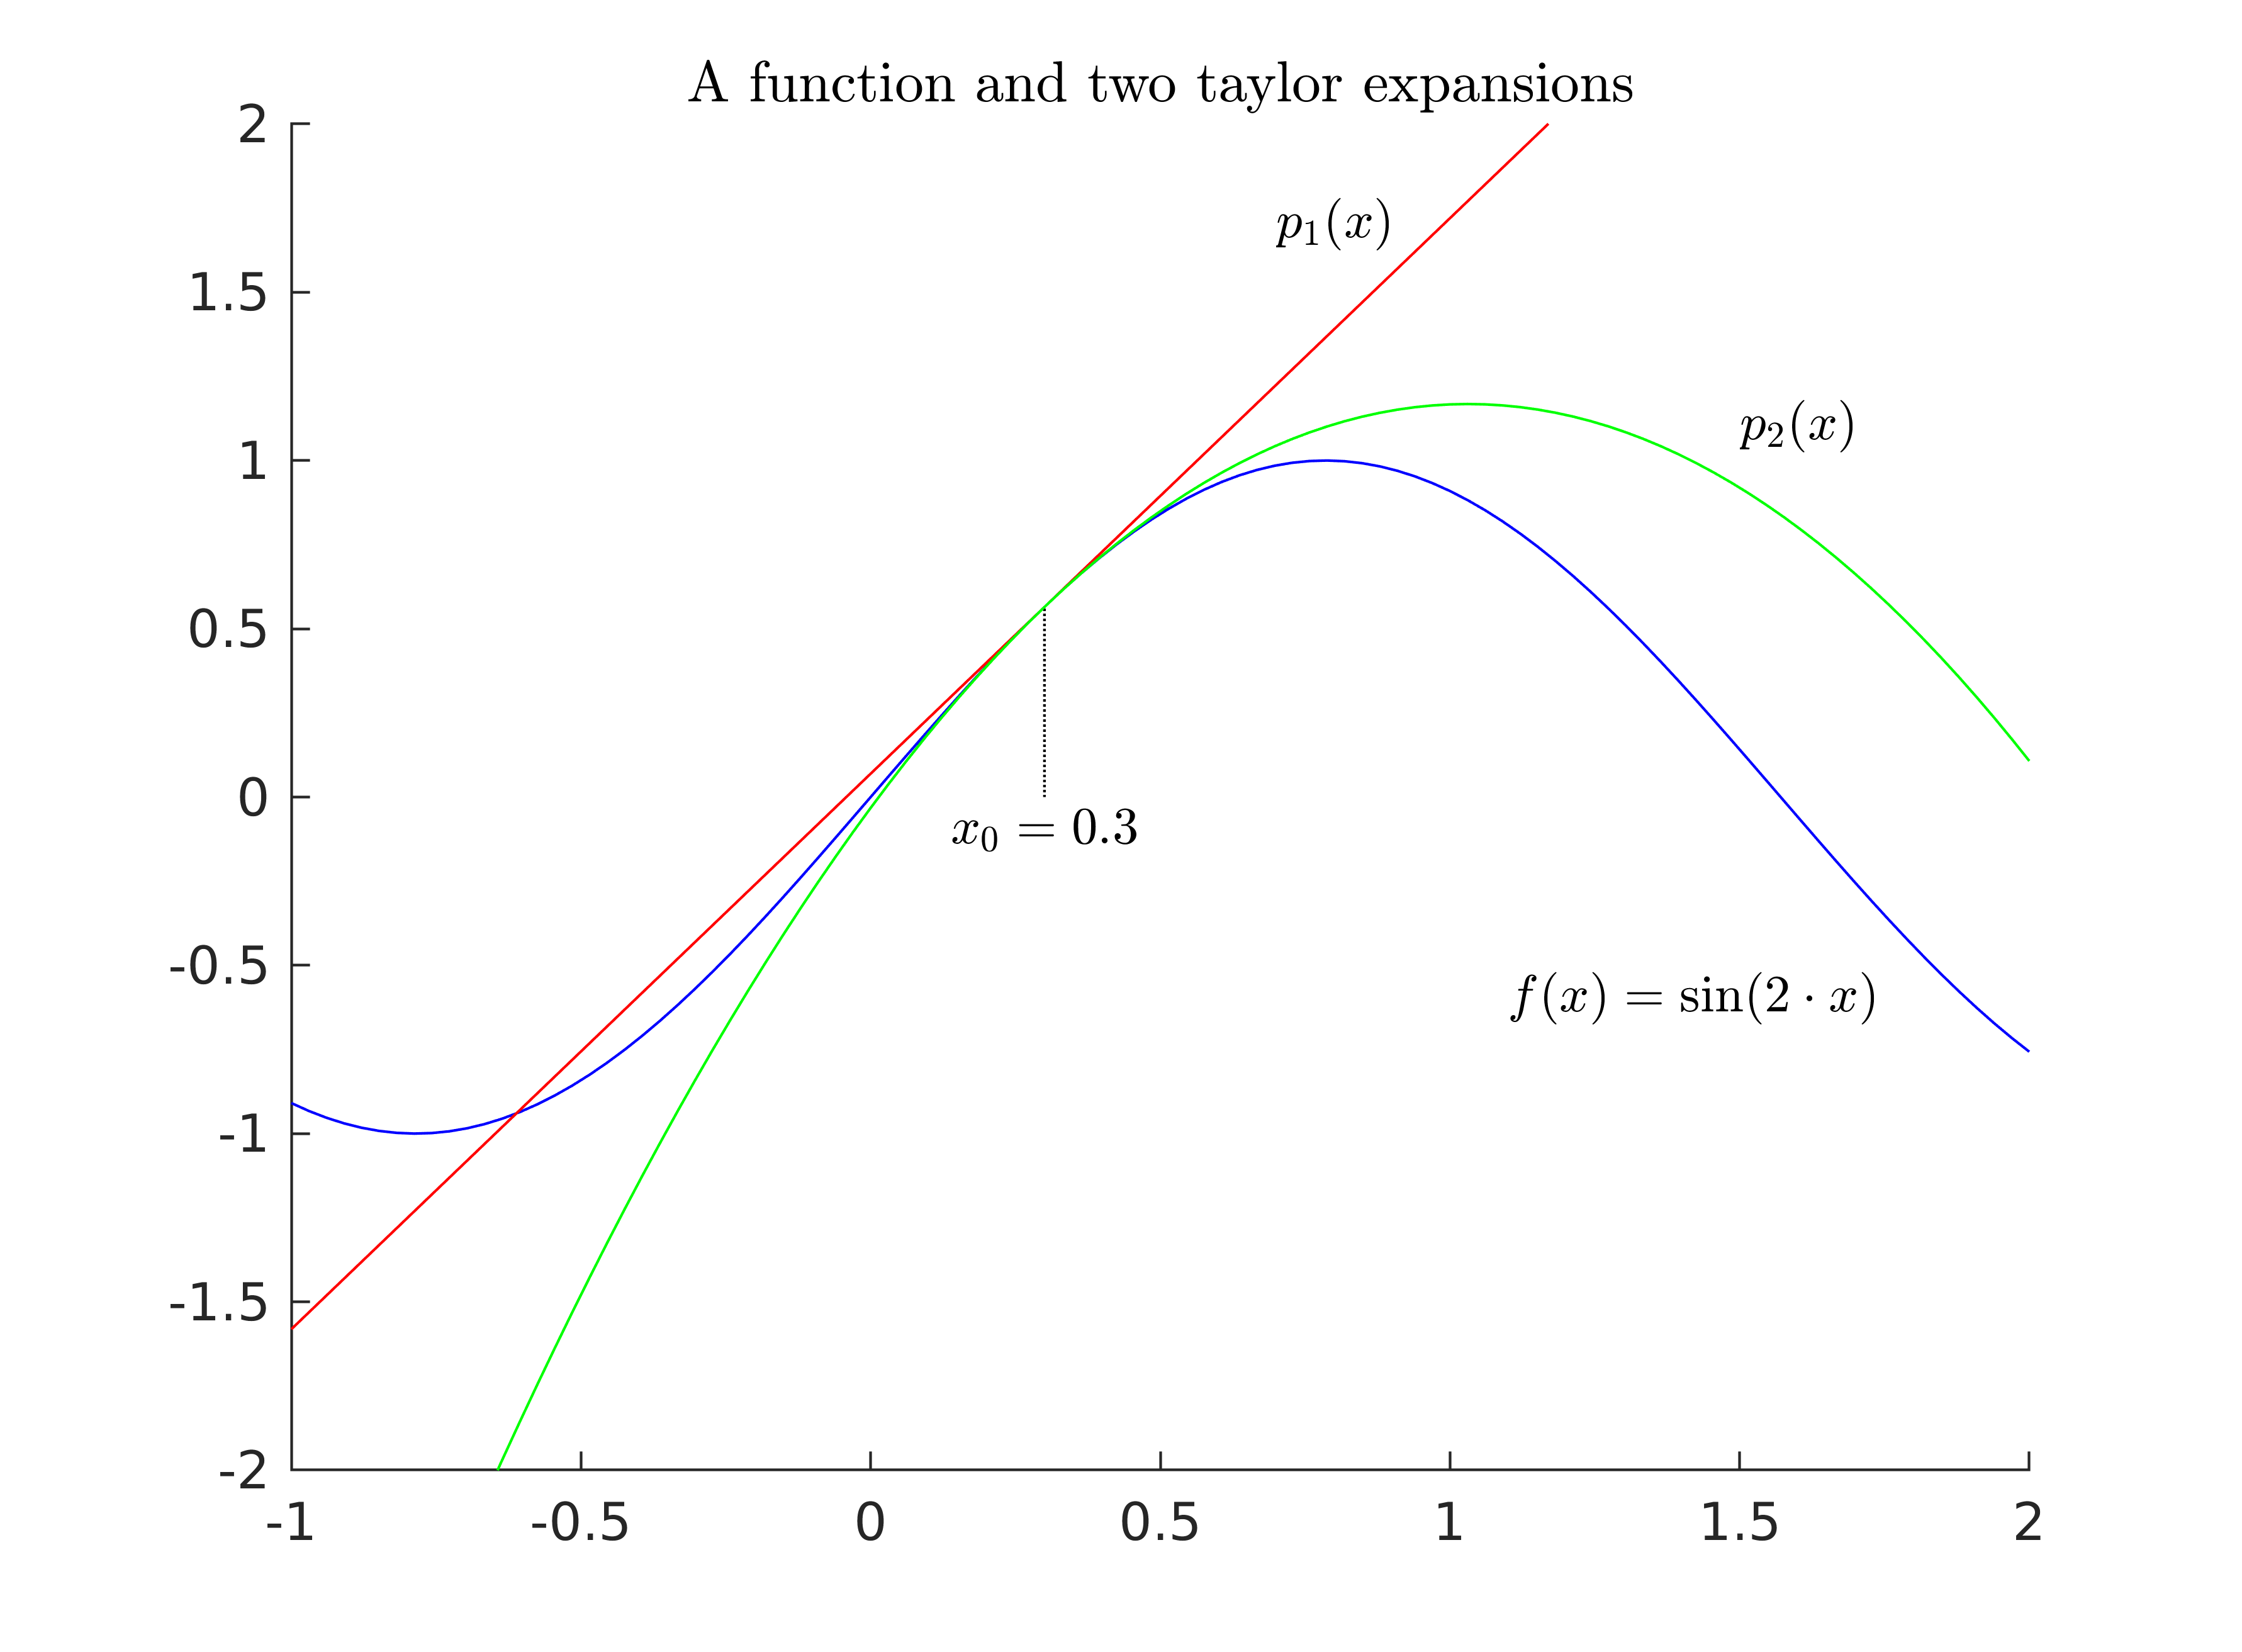
\includegraphics[width=0.7\textwidth]{pic/a_function_and_two_taylorexansions.png}
\end{center}
\begin{hint}
\end{hint}
\begin{sol}
A solution is:
\begin{lstlisting}
%%
xvals = linspace(-1, 2);

fh = @(x) sin(2*x);
dfh = @(x) 2*cos(2*x);
ddfh = @(x) -4*sin(2*x);
x0 = 0.3;

figure(1);
clf;
hold on;
plot(xvals, fh(xvals), 'b')
plot(x0*[1, 1], fh(x0) * [0, 1], 'k:');
plot(xvals, fh(x0)+dfh(x0)*(xvals - x0), 'r')
plot(xvals, fh(x0)+dfh(x0)*(xvals - x0) + 1/2*ddfh(x0)*(xvals - x0).^2, 'g')
ylim([-2, 2])

text(1.1, -0.6, "$f(x) = \sin(2 \cdot x)$", "Interpreter", "latex");
text(0.7, 1.7, "$p_1(x)$", "Interpreter", "latex");
text(1.5, 1.1, "$p_2(x)$", "Interpreter", "latex");
text(0.3, -0.1, "$x_0 = 0.3$", "Interpreter", "latex", ...
     "HorizontalAlignment", "center");
 
title("A function and two taylor expansions", ...
     "Interpreter", "latex");
 
print('a_function_and_two_taylorexansions.png', '-dpng', '-r600');
\end{lstlisting}
\end{sol}
\end{ex}


\begin{ex}
Solve the following five equations with five unknowns:
\begin{align*}
a + b + c + d + e & = 10 \\
a - b + c - d + e & = 6 \\
a + b - c - d - e & = 3 \\
a - b + c & = 3 \\
d + e & = 0
\end{align*}
\begin{hint}
Write the system of equations on extended matrix form
and apply Gaussian elimination.
Then read off the solution.
\end{hint}
\begin{sol}
A solution is:
\begin{lstlisting}
% Enter the linear equations in expanded matrix form.
A = [1, 1, 1, 1, 1, 10; ...
     1, -1, 1, -1, 1, 6; ...
     1, 1, -1, -1, -1, 3; ...
     1, -1, 1, 0, 0, 3; ...
     0, 0, 0, 1, 1, 0];
solution = rref(A)
det(A(:, 1:5))
\end{lstlisting}
\end{sol}
\end{ex}


\begin{ex}
Create a function that calculates the sum of the 
integers from 1 to $n$ raised to a given power $p$.
The function signature should be:
\begin{lstlisting}
function res = sum_of_powers(n, p)
\end{lstlisting}
The input parameters are the last number to include in the 
sum ($n$) and the power to which the integers should be raised ($p$).

The value of \verb!sum_of_powers(4, 3)! is 100
and can be determined through the calculations:
\begin{align*}
\sum_{k = 1}^4 k^3 = 1^3 + 2^3 + 3^3 + 4^3 = 1 + 8 + 27 + 64 = 100
\end{align*}

Use the following examples to test the function:
\begin{lstlisting}
>> sum_of_powers(1, 1)
ans = 1
>> sum_of_powers(4, 1)
ans = 10
>> sum_of_powers(2, 2)
ans = 5
>> sum_of_powers(4, 2)
ans = 30
>> sum_of_powers(10, 1)
ans = 55
>> sum_of_powers(10, 2)
ans = 385
>> sum_of_powers(10, 3)
ans = 3025
\end{lstlisting}
\begin{hint}
\end{hint}
\begin{sol}
A solution is:
\begin{lstlisting}
\end{lstlisting}
\begin{solutionfile}{sum_of_powers_test.m}
%%
function tests = sum_of_powers_test
    tests = functiontests(localfunctions);
end
 

%% Test 1: Positive integer powers of two
function test1(testCase)
    actual_value = sum_of_powers(1, 1);
    expected_value = 1;
    testCase.verifyEqual(actual_value, expected_value);
end

function test2(testCase)
    actual_value = sum_of_powers(1, 2);
    expected_value = 1;
    testCase.verifyEqual(actual_value, expected_value);
end

function test3(testCase)
    actual_value = sum_of_powers(2, 1);
    expected_value = 3;
    testCase.verifyEqual(actual_value, expected_value);
end

function test4(testCase)
    actual_value = sum_of_powers(2, 2);
    expected_value = 5;
    testCase.verifyEqual(actual_value, expected_value);
end

function test5(testCase)
    actual_value = sum_of_powers(10, 1);
    expected_value = 55;
    testCase.verifyEqual(actual_value, expected_value);
end

function test6(testCase)
    actual_value = sum_of_powers(10, 2);
    expected_value = 385;
    testCase.verifyEqual(actual_value, expected_value);
end

function test7(testCase)
    actual_value = sum_of_powers(10, 3);
    expected_value = 3025;
    testCase.verifyEqual(actual_value, expected_value);
end
\end{solutionfile}
\begin{solutionfile}{sum_of_powers.m}
function res = sum_of_powers(n, p)

res = 0;
for k = 1:n
   val = k^p;
   res = res + val;
end

end
\end{solutionfile}
\end{sol}
\end{ex}





% 2020-05-xx
\begin{ex}
Recreate the figure below
\begin{center}
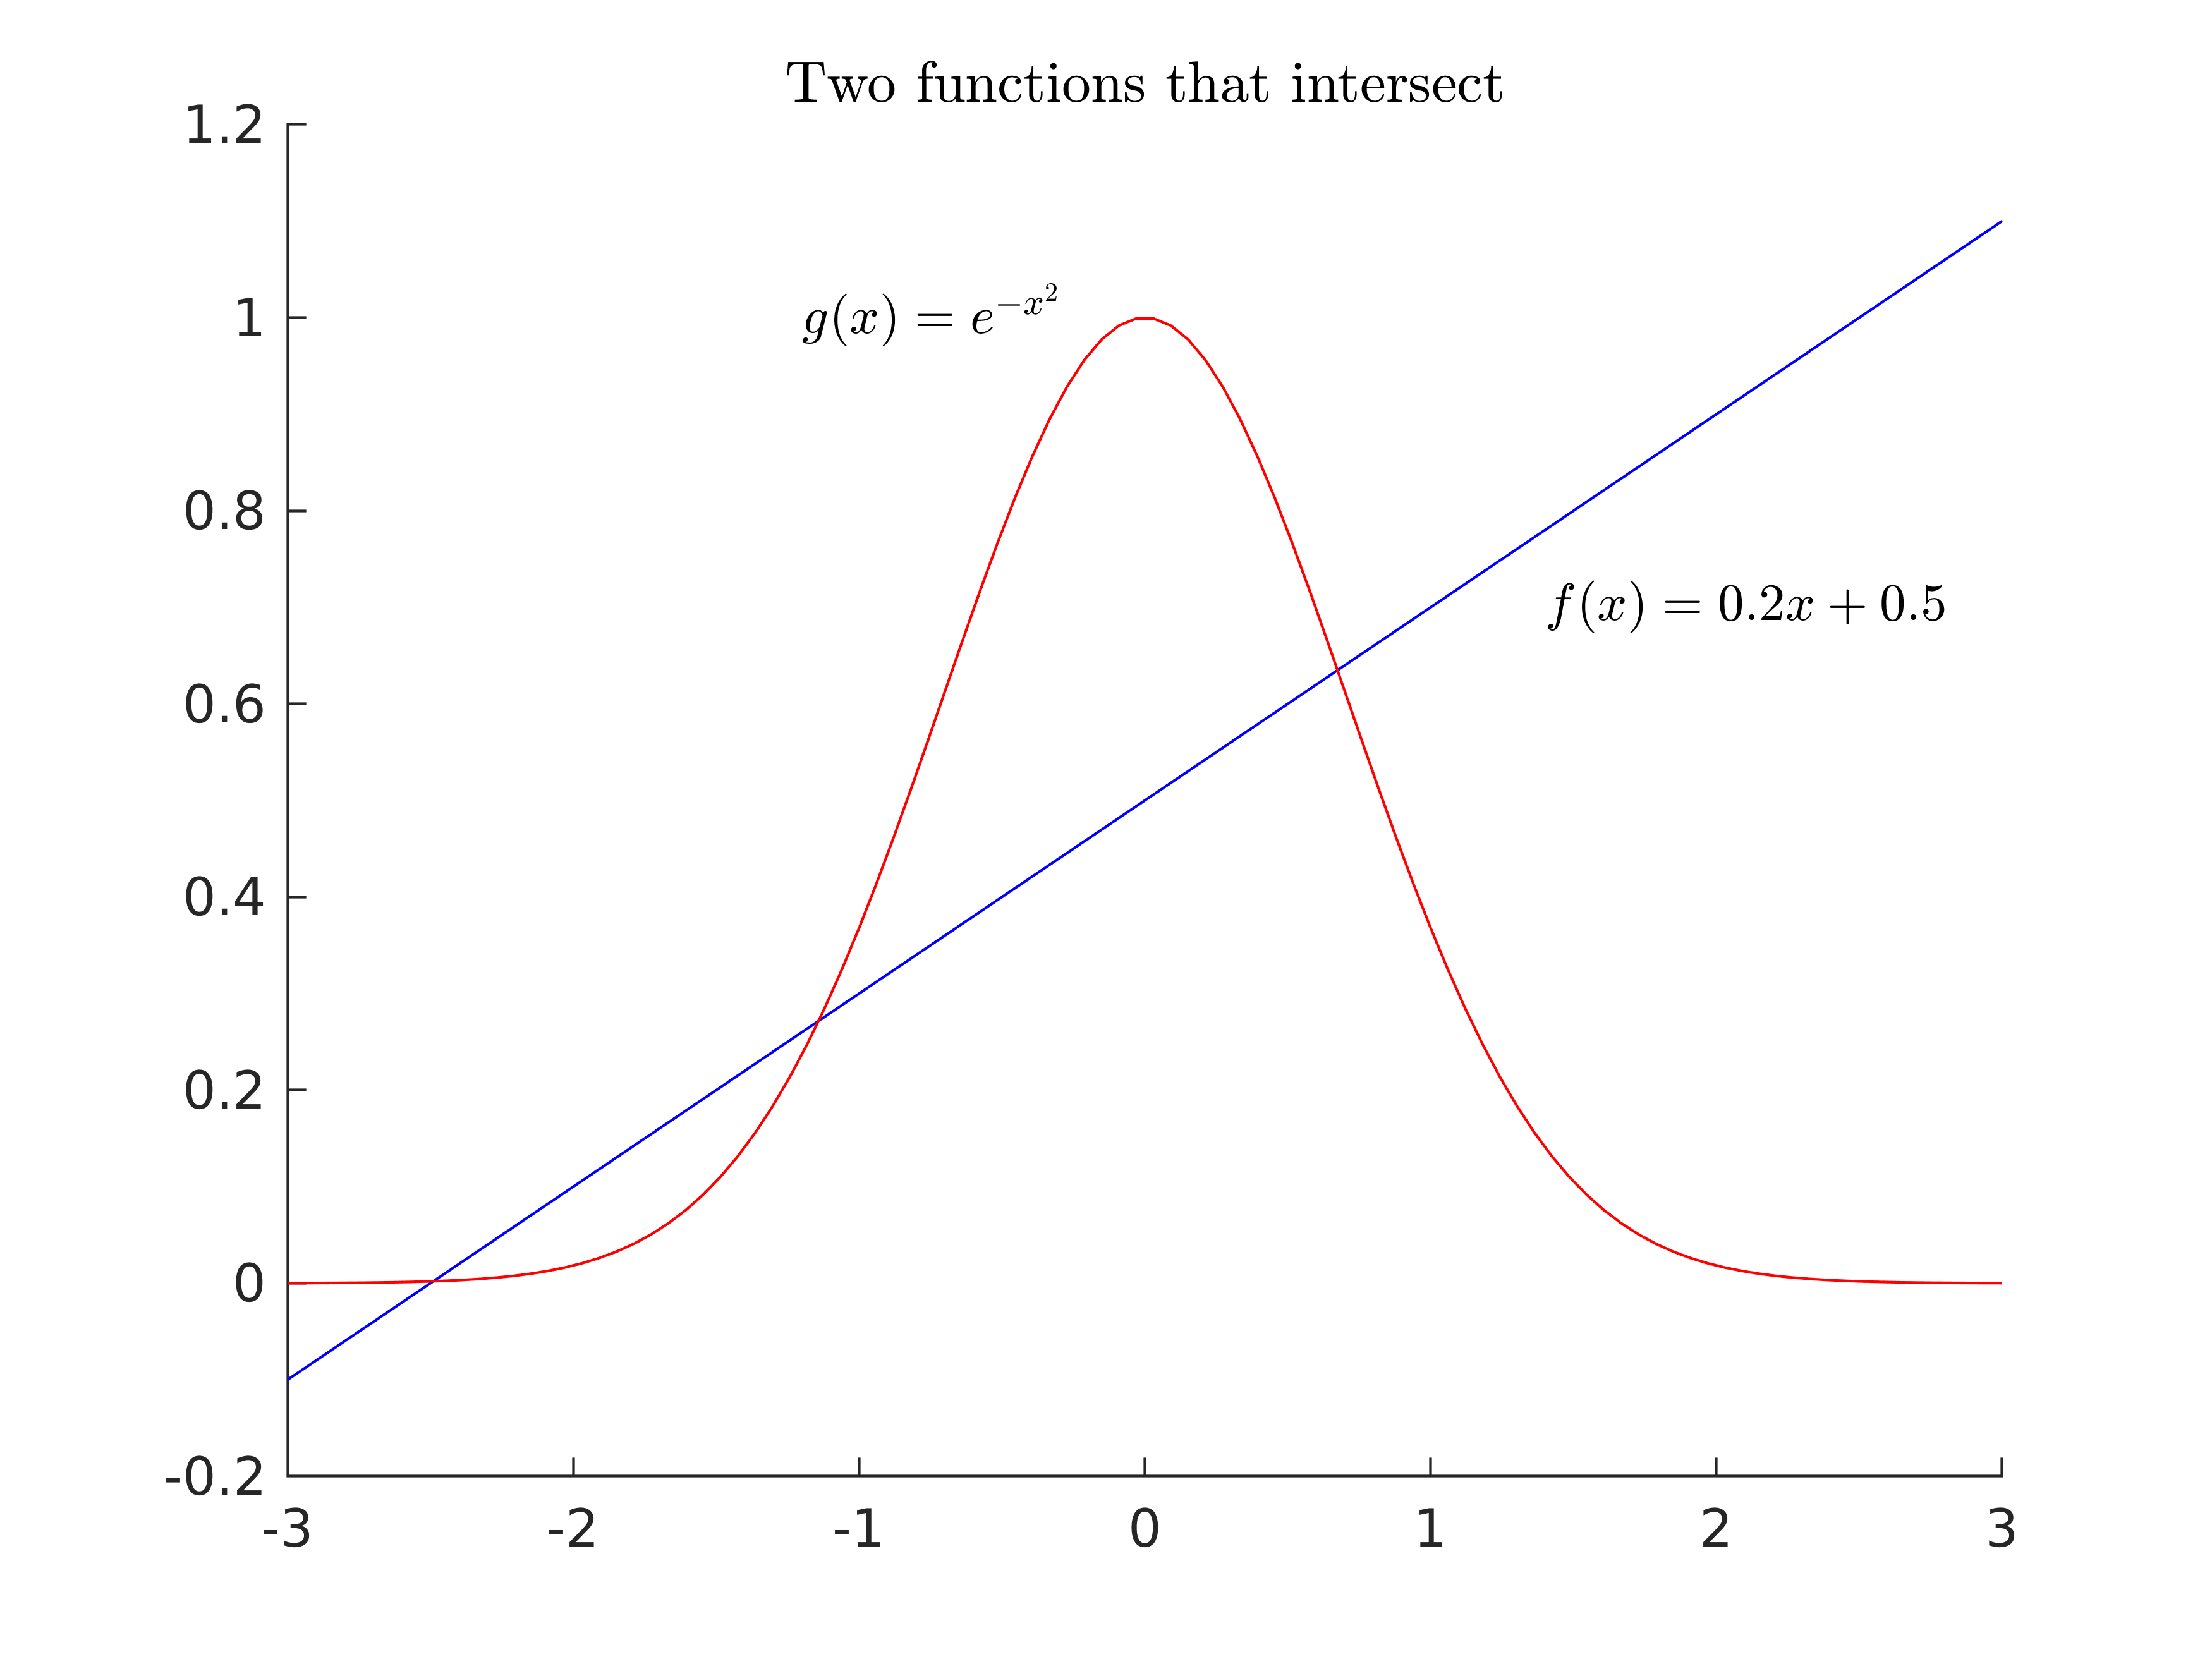
\includegraphics[width=0.7\textwidth]{pic/intersection_of_two_functions.png}
\end{center}
\begin{hint}
\end{hint}
\begin{sol}
A solution is:
\begin{lstlisting}
%%
xvals = linspace(-3, 3);

fh = @(x) 0.2*x + 0.5;
gh = @(x) exp(-x.^2);

figure(1);
clf;
hold on;
plot(xvals, fh(xvals), 'b')
plot(xvals, gh(xvals), 'r')
ylim([-0.2, 1.2])

text(1.4, 0.7, "$f(x) = 0.2 x + 0.5$", "Interpreter", "latex");
text(-1.2, 1.0, "$g(x) = e^{-x^2}$", "Interpreter", "latex");
 
title("Two functions that intersect", ...
     "Interpreter", "latex");
 
print('intersection_of_two_functions.png', '-dpng', '-r600');
\end{lstlisting}
\end{sol}
\end{ex}



\begin{ex}
The following equation has three real solutions:
\begin{align*}
e^{-x^2} = 0.2x + 0.5
\end{align*}
Find these three solutions.
\begin{hint}
\end{hint}
\begin{sol}
A solution is:
\begin{lstlisting}
%%
% Define functions
fh = @(x) 0.2*x + 0.5;
gh = @(x) exp(-x.^2);
hh = @(x) fh(x) - gh(x);

% Search for zeros
r1 = fzero(hh, -2.4)
r2 = fzero(hh, -1)
r3 = fzero(hh, 2)
\end{lstlisting}
\end{sol}
\end{ex}


\begin{ex}
Determine the value of the integral:
\begin{align*}
\int_{-2}^{3} e^{-x^2} dx
\end{align*}
\begin{hint}
\end{hint}
\begin{sol}
A solution is:
\begin{lstlisting}
% Calculate integral
integral(@(x) exp(-x.^2), -2, 3)
\end{lstlisting}
\end{sol}
\end{ex}


\begin{ex}
Implement a function that calculates the area of a triangle 
given the lengths of the three sides using Heron's rule.
Heron's rule is as follows:
Denote the side lengths $a$, $b$ and $c$ and calculate 
the half perimeter:
\begin{align*}
s = \frac{a + b + c}{2}
\end{align*}
Now the area can be calculated through the expression:
\begin{align*}
\textrm{areal} = \sqrt{(s - a) \cdot (s - b) \cdot (s - c) \cdot s}
\end{align*}
The function signature should be:
\begin{lstlisting}
function area = heron(a, b, c)
\end{lstlisting}
The input to the function is the three side lengths
and the value to return is the calculated area.
Eg. is the value of \verb!heron(3, 4, 5)! determined through
the following calculations:
\begin{align*}
s & = \frac{a + b + c}{2} \\ 
& = \frac{3 + 4 + 5}{2} \\
& = 6 \\
\textrm{areal} & = \sqrt{(s - a) \cdot (s - b) \cdot (s - c) \cdot s} \\
& = \sqrt{(6 - 3) \cdot (6 - 4) \cdot (6 - 5) \cdot 6} \\
& = \sqrt{36} = 6
\end{align*}
Use the following examples to test the function:
\begin{lstlisting}
>> heron(3, 4, 5)
ans = 6
>> heron(6, 8, 10)
ans = 24
>> heron(3, 3, 3)
ans = 3.8971
>> heron(3, 3, 6)
ans = 0
>> heron(4, 5, 6)
ans = 9.9216
>> heron(4, 4, 0)
ans = 0
\end{lstlisting}
\begin{hint}
\end{hint}
\begin{sol}
A solution is:
\begin{lstlisting}
\end{lstlisting}
\end{sol}
\end{ex}
 
% !TeX encoding = UTF-8
% !TeX program = pdfLaTeX
% !TeX root = matlab-exercises-emaip.tex
% !TeX spellcheck = en_GB
\section{Functions with if, for and while structures}

\begin{ex}
Create a function which takes a list and a pivot element 
as input. 
Elements in the list that are smaller than the pivot element
should be put in \verb!list1! and elements larger than or equal
should be put in \verb!list2!.
The function signature should be:
\begin{lstlisting}
function [list1, list2] = divide_by_pivot(list, pivot)
\end{lstlisting}
Use the following examples to test the function:
\begin{lstlisting}
>> [l1, l2] = divide_by_pivot([2, 6, 4], 3)
l1 = 2
l2 = 6     4
>> [l1, l2] = divide_by_pivot([2, 6, 4, 1, 4], 7)
l1 = 2     6     4     1     4
l2 = []
>> [l1, l2] = divide_by_pivot([2, 6, 4, 1, 4], 3)
l1 = 2     1
l2 = 6     4     4
\end{lstlisting}
\begin{hint}
Use a for loop to iterate over all elements in the input 
list.
Use an if statement to select which list the element should 
be added to.
\end{hint}
\begin{sol}
A solution is:
\begin{lstlisting}
function [list1, list2] = divide_by_pivot(list, pivot)

list1 = [];
list2 = [];
for val = list
    if val < pivot
        list1 = [list1, val];
    else
        list2 = [list2, val];
    end
end

end
\end{lstlisting}
\end{sol}
\end{ex}

\begin{ex}
Create a function that takes a list as input.
All elements in the list larger than zero should 
be put in a list that is then returned.

The function signature should be:
\begin{lstlisting}
function list = keep_positive_elements(input_list)
\end{lstlisting}
Use the following examples to test the function:
\begin{lstlisting}
>> keep_positive_elements([1, -2, 3, -4, 5])
ans = 1     3     5
>> keep_positive_elements([-1, -2, -3, -4, 5])
ans = 5
>> keep_positive_elements([6, 4, 2, 1])
ans = 6     4     2     1
\end{lstlisting}
\begin{hint}
Use a for loop to iterate over all values in 
the input list.
Use an if statement to decide whether the value
should be added to the output.
\end{hint}
\begin{sol}
A solution is:
\begin{lstlisting}
function list = keep_positive_elements(input_list)

list = [];
for val = input_list
    if val > 0
        list = [list, val];
    end
end

end
\end{lstlisting}
\end{sol}
\end{ex}


\begin{ex}
Create a function that takes a list of $n$ points as input 
(in the form of a $n$ by $2$ matrix).
The function should return a matrix with distances between 
the input points, so the element $a_{12}$ in the matrix 
contains the distance between the first and the second point
in the input list.
The function signature should be:
\begin{lstlisting}
function res = distance_matrix(list_of_points)
\end{lstlisting}
Use the following examples to test the function:
\begin{lstlisting}
>> distance_matrix([1, 0; 1, 1])
ans =
     0     1
     1     0
>> distance_matrix([1, 0; 0, 1; 1, 1])
ans =
         0    1.4142    1.0000
    1.4142         0    1.0000
    1.0000    1.0000         0
>> distance_matrix([1, 0; 1, 1; 4, 4])
ans =
         0    1.0000    5.0000
    1.0000         0    4.2426
    5.0000    4.2426         0
\end{lstlisting}
\begin{hint}
To calculate the distance matrix, all combinations
of two points should be examined.
This can be achieved by using two for loops placed 
inside each other (so you have an outer loop and an 
inner loop).
\end{hint}
\begin{sol}
A solution is:
\begin{lstlisting}
function res = distance_matrix(list_of_points)

[s1, s2] = size(list_of_points);
res = zeros(s1, s1);

for idx1 = 1:s1
    for idx2 = 1:s1
        p1 = list_of_points(idx1, :);
        p2 = list_of_points(idx2, :);
        difference = p1 - p2;
        distance = norm(difference);
        res(idx1, idx2) = distance;
    end
end

end
\end{lstlisting}
\end{sol}
\end{ex}


\begin{ex}
Create a function which takes two lists as input.
The output should be the two lists combined, 
so that all elements in the first list appears
before all elements in the second list.

The function signature should be:
\begin{lstlisting}
function res = concatenate_lists(list1, list2)
\end{lstlisting}
Use the following examples to test the function:
\begin{lstlisting}
>> concatenate_lists([1, 2, 3], [4, 5])
ans =
     1     2     3     4     5
>> concatenate_lists([5, 4], [1, 2, 3])
ans =
     5     4     1     2     3
\end{lstlisting}
\begin{hint}
Use a while loop to move all elements from list1 
to the output list.
Then use a new while loop to move all elements from 
list2 to the output list.
\end{hint}
\begin{sol}
A solution is:
\begin{lstlisting}
function res = concatenate_lists(list1, list2)

res = [];
idx = 1;
while idx <= length(list1)
    res = [res, list1(idx)];
    idx = idx + 1;
end

idx = 1;
while idx <= length(list2)
    res = [res, list2(idx)];
    idx = idx + 1;
end

end
\end{lstlisting}
\end{sol}
\end{ex}


\begin{ex}
\label{exSecantMethodOneStep}%
Implement a function that takes a function handle, and two 
$x$ values.
Use one step of the secant method to make an improved guess of the
root of a function, by using the two $x$ values as guesses.
The calculation to be done in the function is the following
where $f(x)$ is the function specified by the function handle
applied to the value $x$, and $x_1$ and $x_2$ are the two
guesses.
\[
x=x_{2}-f(x_{2}) \cdot {\frac {x_{2}-x_{1}}{f(x_{2})-f(x_{1})}}.
\]
You can read more about the secant method on \href{https://en.wikipedia.org/wiki/Secant_method}{wikipedia}.

The function signature should be:
\begin{lstlisting}
function [x_improved, fval] = sekant_one_step(fh, x1, x2)
\end{lstlisting}
Use the following examples to test the function:
\begin{lstlisting}
>> [x, v] = sekant_one_step(@cos, 1, 2)
x = 1.5649
v = 0.0059
>> [x, v] = sekant_one_step(@cos, 2, 1.5649)
x = 1.5710
v = -1.8238e-04
>> [x, v] = sekant_one_step(@tan, 3, 3.5)
x = 3.1378
v = -0.0038
>> [x, v] = sekant_one_step(@tan, 3.5, 3.1478)
x = 3.1419
v = 2.7253e-04
\end{lstlisting}
\begin{hint}
No if, for or while loop is needed in this exercise.
\end{hint}
\begin{sol}
A solution is:
\begin{lstlisting}
function [x_improved, fval] = sekant_one_step(fh, x1, x2)

fx1 = fh(x1);
fx2 = fh(x2);

slope = (fx2 - fx1) / (x2 - x1);

x_improved = x2 - fx2 / slope;
fval = fh(x_improved);

end
\end{lstlisting}
\end{sol}
\end{ex}


\begin{ex}
Implement a function which takes a function handle, two $x$ 
values and a limit value as input.
Use the function implemented in exercise
\ref{exSecantMethodOneStep} to improve the root estimates.
Apply the function until the absolute value of the function 
evaluated at the best guess gets below the limit value.
Then return the improved guess, the value of the function 
evaluated at that guess and the number of
iterations used.

The function signature should be:
\begin{lstlisting}
function [x1, fvalue, iterations] = ...
    sekant_method(fh, x0, x1, limit)
\end{lstlisting}
Use the following examples to test the function:
\begin{lstlisting}
>> [x, fval, niter] = sekant_method(...
    @cos, 1.2, 2, 0.01)
x = 1.5724
fval = -0.0016
niter = 1
>> [x, fval, niter] = sekant_method(...
    @sin, 3, 4, 0.01)
x = 3.1395
fval = 0.0021
niter = 2
>> [x, fval, niter] = sekant_method(...
    @sin, 3, 4, 0.001)
x = 3.1416
fval = -7.4395e-08
niter = 3
>> [x, fval, niter] = sekant_method(...
    @(x) log(x) - 1, 3, 4, 0.001)
x = 2.7184
fval = 5.6055e-05
niter = 3
\end{lstlisting}
\begin{hint}
Use a while loop to repeat the calculations as many times 
as needed until the function value gets below the 
specified limit value.
\end{hint}
\begin{sol}
A solution is:
\begin{lstlisting}
function [x1, fvalue, iterations] = sekant_method(fh, x0, x1, limit)

iterations = 0;
fvalue = fh(x1);
while abs(fvalue) > limit
    [x2, fvalue] = sekant_one_step(fh, x0, x1);
    x0 = x1;
    x1 = x2;
    iterations = iterations + 1;
end

end
\end{lstlisting}
\end{sol}
\end{ex}


\begin{ex}
Implement a function that takes two lists
with numerical values as input.
Both lists are sorted, so their values are in 
increasing order.
The two lists should be merged together
in a single list such that the values in 
that list is also sorted.

The function signature should be:
\begin{lstlisting}
function res = merge_ordered_lists(list1, list2)
\end{lstlisting}
Use the following examples to test the function:
\begin{lstlisting}
>> merge_ordered_lists([1, 2, 4], [3, 7, 8])
ans = 1     2     3     4     7     8
>> merge_ordered_lists([1, 2, 4], [])
ans = 1     2     4
>> merge_ordered_lists([], [1, 2, 4])
ans = 1     2     4
\end{lstlisting}
\begin{hint}
Use three while loops.
The first while loop extracts the lowest value from 
the two lists and inserts it in the result.
The loops ends when all values have been used from 
one of the lists.
The second while loop moves all the remaining elements 
in list one to the result.
The third while loop moves all the remaining elements 
in list two to the result.
\end{hint}
\begin{sol}
A solution is:
\begin{lstlisting}
function res = merge_ordered_lists(list1, list2)

res = [];
idx1 = 1;
idx2 = 1;

while idx1 <= length(list1) && idx2 <= length(list2)
    if list1(idx1) < list2(idx2)
        res = [res, list1(idx1)];
        idx1 = idx1 + 1;
    else
        res = [res, list2(idx2)];
        idx2 = idx2 + 1;
    end
end

while idx1 <= length(list1)
    res = [res, list1(idx1)];
    idx1 = idx1 + 1;
end

while idx2 <= length(list2)
    res = [res, list2(idx2)];
    idx2 = idx2 + 1;
end

end
\end{lstlisting}
\end{sol}
\end{ex}



\begin{ex}
Create a function that takes a list of points and a query point
as input.
The function should then determine the point from the 
input list that is nearest the query point.
The index of the nearest point and the distance to the 
query point should then be returned.

The function signature should be:
\begin{lstlisting}
function [min_dist_idx, min_distance] = ...
    locate_nearest_point(input_list, query_point)
\end{lstlisting}
Use the following examples to test the function:
\begin{lstlisting}
>> [idx, dist] = locate_nearest_point([1, 1; 1, 5], [1.1, 1])
idx = 1
dist = 0.1000
>> [idx, dist] = locate_nearest_point([1, 1; 1, 5; 5, 4], [2, 4])
idx = 2
dist = 1.4142
>> [idx, dist] = locate_nearest_point([1, 1; 1, 5], [2, 4])
idx = 2
dist = 1.4142
\end{lstlisting}
\begin{hint}
Use a for loop to iterate over all points in the list of points.
For each point in the list, calculate the distance to the 
reference point and save the index of the point and the
distance to it, if it is the smallest distance seen thus far.
\end{hint}
\begin{sol}
A solution is:
\begin{lstlisting}
function [min_dist_idx, min_distance] = ...
    locate_nearest_point(input_list, query_point)

min_dist_idx = -1;
min_distance = 100000000;

for idx = 1:size(input_list, 1)
    point = input_list(idx, :);
    difference = point - query_point;
    distance = norm(difference);
    if distance < min_distance
        min_dist_idx = idx;
        min_distance = distance;
    end
end

end
\end{lstlisting}
\end{sol}
\end{ex}
 
% !TeX encoding = UTF-8
% !TeX program = pdfLaTeX
% !TeX root = matlab-exercises-emaip.tex
% !TeX spellcheck = en_GB
\section{The min heap data structure}

\todo[inline]{Create exercise: is\_min\_heap(list)}
\todo[inline]{Create exercise: build\_heap(list)}
\todo[inline]{Create exercise: is\_sorted(list)}
\todo[inline]{Create exercise: heap\_sort(list)}

Code examples are available here: 
2020-09-01\_EMAIP/materialer/matlablectures/test/getting-started-with-matlab-with-unittests/22\_more\_functions
 
% !TeX encoding = UTF-8
% !TeX program = pdfLaTeX
% !TeX root = matlab-exercises-emaip.tex
% !TeX spellcheck = en_GB
\section{How to solve second order differential equations numerically}

Fortæl om ode45 og giv eksempler pá brug ap denne solver. Naun også deval
Vis huordan ct andet ordens differentiol ligning kan omsknies tic to koblede forste ordens diffferential liqninger.
\begin{align*}
y^{\prime \prime}=f\left(x, y, y^{\prime}\right)
\end{align*}
Introducer \(\quad V=y^{\prime} \rightarrow v^{\prime}=y^{\prime \prime}\)
\begin{align*}
v^{\prime}&=f(x, y, v) \\
y^{\prime}&=\ddot{v}^{\prime}
\end{align*}
Nu er der to ligninger der er koblede.

Vis hvordan de lases numen'st.
 
% !TeX encoding = UTF-8
% !TeX program = pdfLaTeX
% !TeX root = matlab-exercises-emaip.tex
% !TeX spellcheck = en_GB
\section{Numerical root finding}

\todo[inline]{Add exercises about plotting phase space diagrams for differential equations}
\todo[inline]{Examine the stability about equilibria in differential equations}

In the next set of exercises the goal will be to find solutions to the equation
%
\begin{align}
x
	& = \exp(x - 2)
\end{align}
%
The first step is to rewrite the equation such that one of the sides become 0.
%
\begin{align}
0
	& = \exp(x - 2) - x
\end{align}
%
The right hand side will be denoted $f(x)$ and the problem is now to find the 
roots of the function $f(x)$.
\begin{align}
0 & = f(x)
\end{align}

\begin{ex}
Locate the two roots of the function graphically using the plot command in matlab.
To ensure precise readings use the zoom functionality.
Give the roots with at least three correct decimals.
\end{ex}


\subsection{Fixed point iteration}

\begin{align}
f_0(x_0)
	& = f(x_0)	\\
f_n(x_0)
	& = f_{n - 1}(x_0)
\end{align}


\begin{ex}
Create a function which performs fixed point iterations on a given
function.
The function should take three input arguments, a function handle $f$, the initial x value 
($x_0$) and the number of iterations ($n$).
The return value should be $f_n(x_0)$.
The intermediate calculations $f_0(x_0)$, $f_1(x_0)$, $f_2(x_0)$, \ldots 
should be displayed on screen.

\begin{lstlisting}
function res = fixedIter(x0, n)
\end{lstlisting}
Example usage of the function:
\begin{lstlisting}
>> fnc = @(x) exp(x - 2);
>> fixedIter(fnc, 1, 2)
    0.3679
    0.1955
    0.1646
ans =
    0.1646
\end{lstlisting}
\end{ex}

\begin{ex}
Does the function fixedIter always converge to the same value when used on the function
handle given in the exercise above?
If the function converges, how is the converged value related 
to the equation $x = \exp(x - 2)$?
\end{ex}




\begin{ex}
Implement a function which uses bisection to locate roots in a given function. 
As input should it take a function handle, the initial interval (given as 
lower and higher values) and the number of iterations.
If the function have opposite signs at the lower and higher values the 
bisection method should run, in the other case a warning should be issued.
As output the function should return an array containing four columns and a number of 
rows equal to the number of iterations.
Each row should have the values \emph{lower}, \emph{higher}, \emph{fvalLower} and 
\emph{fvalHigher} (the current limits and the function values at the limits).
 
\begin{lstlisting}
function data = bisection(fnc, lower, higher, iterations)
\end{lstlisting}
Example usage of the function:
\begin{lstlisting}
>> fnc = @(x) exp(x - 2) - x;
>> bisection(fnc, 0, 0.1, 5)
Bad starting values
ans =[]
>> bisection(fnc, 0, 1, 5)
ans =
         0    0.5000    0.1353   -0.2769
         0    0.2500    0.1353   -0.0762
    0.1250    0.2500    0.0284   -0.0762
    0.1250    0.1875    0.0284   -0.0243
    0.1563    0.1875    0.0020   -0.0243
\end{lstlisting}
\end{ex}


\begin{ex}\\
Investigate how the bisection method converges. 
E. g. how many iterations is required to reach a given accuracy?
\end{ex}

\begin{ex}
Implement a function which uses the secant method to locate roots in a given function.
As input should it take a function handle and two different $x$ values near the root 
that should be located and the number of iterations.
If the method converges before the requested number of iterations it should halt 
(the method has converged when the calculated function value is zero).
After each iteration the method should output the new estimate of the root location $x$
and the function value at $x$.
The secant method is described here \url{http://en.wikipedia.org/wiki/Secant_method}.

\begin{lstlisting}
function secant(fnc, x0, x1, iterations)
\end{lstlisting}
Example usage of the function:
\begin{lstlisting}
>> fnc = @(x) exp(x - 2) - x;
>> format long
>> secant(fnc, 3, 3.4, 3)
   3.400000000000000   0.655199966844675
   3.120274401785570  -0.054579081629965
   3.141784146672724  -0.009432188618255
>> secant(fnc, 0.1, 0.2, 9)
   0.200000000000000  -0.034701111778413
   0.158821380623629  -0.000191029545640
   0.158593437586678   0.000000758928080
   0.158594339582341  -0.000000000016240
   0.158594339563039                   0
\end{lstlisting}
\end{ex}



\begin{ex}\\
Implement a function which uses the regula falsi method locate roots in a given function.
As input should it take a function handle, the initial interval (given as 
lower and higher values) and the number of iterations.
If the function has opposite signs at the lower and higher values the 
regula falsi method should run, in the other case a warning should be issued.
As output the function should return an array containing four columns and a number of 
rows equal to the number of iterations.
Each row should have the values \emph{lower}, \emph{higher}, \emph{fvalLower} and 
\emph{fvalHigher} (the current limits and the function values at the limits).

\begin{lstlisting}
function regulafalsi(fnc, lower, higher, iterations)
\end{lstlisting}
Example usage of the function:
\begin{lstlisting}
>> fnc = @(x) exp(x - 2) - x;
>> regulafalsi (fnc, 0 ,  -1,  5)
Bad starting values
ans = []
>> regulafalsi (fnc, 0 ,  0.1,  5)
Bad starting values
ans = []
>> regulafalsi (fnc, 0 ,  1,  4)
ans =
         0    0.1763    0.1353   -0.0149
         0    0.1588    0.1353   -0.0002
         0    0.1586    0.1353   -0.0000
         0    0.1586    0.1353   -0.0000
>> result = regulafalsi (fnc, -10 ,  1,  5)
result =
  -10.0000    0.3460   10.0000   -0.1547
  -10.0000    0.1884   10.0000   -0.0250
  -10.0000    0.1630   10.0000   -0.0037
  -10.0000    0.1592   10.0000   -0.0005
  -10.0000    0.1587   10.0000   -0.0001
\end{lstlisting}
\end{ex}

\begin{ex}\\
Is the regula falsi method working well in the example given above? 
Try to compare with the convergence of the bisection method, which converges 
most quickly?
Try to suggest a combination of the two methods that will converge faster than 
either bisection and regula falsi.
\end{ex}



\begin{ex}\\
Create a function which implements Newtons method. 
As input should it take two function handles (one for $f(x)$ and one for $f'(x)$), 
an initial guess $x_0$ and the number of iterations.
As output should it return a list of the calculated $x$ values, one value for each performed iteration.
\begin{lstlisting}
function result = newton(fnc, dfnc, x0, iterations )
\end{lstlisting}
Example usage of the function:
\begin{lstlisting}
>> fnc = @(x) cos(x);
>> dfnc = @(x) - sin(x);
>> format long;
>> vals = newton(fnc, dfnc, 1, 2)
vals = 1.000000000000000   1.642092615934331   1.570675277161251
\end{lstlisting}
\end{ex}




\begin{ex}\\
Compare the convergence properties of the implemented functions for rootfinding, 
ie how many iterations are required to reach a function value below $10^{-1}$,
$10^{-2}$, $10^{-4}$, $10^{-8}$, $10^{-12}$\,?

Use the following equation as case: $f(x) = \exp(x - 4) + \cos(x)$.
As initial values use $x_0 = 5$ for Newtons method and the ends of the range 
$x \in [2; 5]$ for the methods requiring two initial values.
Make table like the one below, which contains the number of iterations used for 
each method to find a function value less than a given threshold.

\begin{centering}
\begin{tabular}{l|r|r|r|r|r}
Method \textbackslash Function value	& $10^{-1}$ & $10^{-2}$ & $10^{-4}$ & $10^{-8}$ & $10^{-12}$ \\
\hline
Newton	&  	& 3 	&  	&  	&	\\
Secant	& 4	&	& 	& 	&	\\
Bisection	&	&	&	&	&	\\
Regula falsi &	&	&	& 	& 36	\\
\end{tabular}
\end{centering}
\end{ex}
 


\section{Plotting}

To plot eg. the sine function in matlab, the following code
can be used:
\begin{lstlisting}
% Open figure 1
figure(1);

% Clear the content of figure one (this only have an effect 
% if figure 1 already contained previously plotted material)
clf;

% Generate a list of x values, for which the function should be 
% plotted.
x = linspace(-2, 7);

% Plot the function
plot(x, sin(x));
\end{lstlisting}

\subsection{Plotting multiple things in the same plot}

By default matlab will overwrite the content of a figure
when a new plot command is issued.
So for instance if you want to plot both the sine and the cosine 
function in the same plot, this approach would fail, as only the 
cosine function will be present in the generated plot.

\begin{lstlisting}
figure(1);
clf; 
x = linspace(-2, 7);
plot(x, sin(x));
plot(x, cos(x));
\end{lstlisting}

To plot multiple things in the same plot, matlab should be told
to keep using the same ``paper'' that the plot is drawn upon.
This is achieved by the \verb!hold on! command.
After a \verb!hold on! command is issued, matlab will not erase 
the content of a plot but will add new material to the plot.

\begin{lstlisting}
figure(1);
clf; 
x = linspace(-2, 7);
plot(x, sin(x));
hold on;
plot(x, cos(x));
\end{lstlisting}

The plot can be taken out of the \verb!hold on! state, by the 
command \verb!hold off! or by clearing the figure using the 
command \verb!clf!.


\subsection{Adding information to plots}
\label{ssecAddingInformationToPlots}

It is often beneficial to add some text to plots, 
that can describe what is visualized and what are on the 
axes. 
This can be achieved using the commands \verb!title!, 
\verb!xlabel! and \verb!ylabel! as shown here:
\begin{lstlisting}
title("Harmonic oscillations")
xlabel("Time [s]")
ylabel("Offset")
\end{lstlisting}

If you need to add mathematical expression it is possible 
for matlab to visualise latex expressions.
To do this specify that the latex interpreter is used when 
formatting text as shown here:
\begin{lstlisting}
title("Harmonic oscillations $a^b$", 'interpreter', 'latex')
xlabel("Time $t$ [s]", 'interpreter', 'latex')
ylabel("Offset $\sin(t)$", 'interpreter', 'latex')
\end{lstlisting}


\subsection{Specifying plot limits}

For some plots it is only of interest to show a specific 
part of the coordinate system.
To choose which part to include in a plot, use the 
\verb!xlim! and \verb!ylim! commands.


\subsection{Adding text annotations to a plot}

Text elements can be placed in the plot area
using the \verb!text! command.
The command requires three arguments, the location of the 
text specified as $x$ and $y$ coordinates and the 
text to insert.
It is also possible to insert mathematical expressions
using the \verb!text! command as described in 
\ref{ssecAddingInformationToPlots}.


\subsection{Multiple plots in each figure}

On information about how to add multiple
plots to a single figure, see section 
\ref{ssecMultiplePlotsInOne}.



\section{Random number generation}

Matlab is able to generate random numbers.
This can be practical in multiple situations.
The random numbers are created by a random number 
generator, which is able to generate numbers that 
(at least) appear to be random, even if a computer 
has generated them.

To simulate a six sided dice, the \verb!randi! command
can be used.
\begin{lstlisting}
>> randi(5)
ans = 3
>> randi(5)
ans = 4
\end{lstlisting}
If a matrix filled with random values are needed, the size
of the matrix can be specified to \verb!randi! as shown here:
\begin{lstlisting}
>> randi(5, 2, 4)
ans = 5     4     3     1
      1     3     1     5
\end{lstlisting}

Similarly can you get a random number from a uniform 
distribution between zero and one by using the \verb!rand! 
function.
\begin{lstlisting}
>> rand()
ans = 0.6385
>> rand()
ans = 0.0336
\end{lstlisting}
In some cases it is beneficial to be able to produce the exact
same sequence of ``random numbers'' multiple times.
This can be achieved by setting the state of the random number 
generator, which is done as follows:
\begin{lstlisting}
>> rng(1); 
>> randi(10, 1, 5)
ans = 5     8     1     4     2
\end{lstlisting}

\subsection{Using random numbers}

One case for using random numbers is to generate 
calculation exercises. 
Below is an example that generates a system of three
equations with three unknowns in the form 
$A \cdot \vec{x} = \vec{b}$.
The system of equations are generated by populating 
$A$ and $\vec{x}$ with random integers.
Then their product is calculated and finally are
$A$ and $\vec{b}$ shown to the user.
\begin{lstlisting}
n = 3;
A = randi([-3, 3], [n, n])
x = randi([-5, 5], [n, 1]);
b = A*x
\end{lstlisting}
The generated output could look like
\begin{lstlisting}
A =  3     3    -3
    -1     3    -2
     1    -3     3
b = -30
     -9
     14
\end{lstlisting}



\section{Loose ends}


\todo[inline]{Add exercises about secret sharing. Get inspiration from this video: Secret Sharing Explained Visually \url{https://www.youtube.com/watch?v=iFY5SyY3IMQ}}

\todo[inline]{Add exercise on implementing a perceptron, \url{https://www.khanacademy.org/computer-programming/perceptron-classifier/993241235}}

\todo[inline]{Matlab exercise on implementing quicksort and other sorting algorithms}

\todo[inline]{Lav en opgave om at finde modstande (og kombinationer af disse) der er tættest på en ønsket værdi}


\todo[inline]{Lav en opgave om fordeling af mandater ud fra antal afgivne stemmer vha. den Hondske metode
\href{https://da.wikipedia.org/wiki/D\%27Hondts_metode}{wikipedia}}

\todo[inline]{Lav en opgave om at lave slope plots i matlab.}

\Closesolutionfile{hnt}
\Closesolutionfile{ans}


\newpage
\section{Hints}
\input{hints}


\newpage
\section{Solutions}
\input{ans}


\newpage
\section{Links to other resources}

Beginning Matlab Exercises, by R. J. Braun: 
\url{http://www.math.udel.edu/~braun/M349/Matlab_probs2.pdf}

\url{http://kom.aau.dk/~borre/matlab7/exercise.pdf}


\end{document}
